\documentclass[conference]{IEEEtran}
\IEEEoverridecommandlockouts

\usepackage{amsmath,amssymb,amsfonts}
\usepackage{algorithmic}
\usepackage{graphicx}
\usepackage{textcomp}
\usepackage{xcolor}
\usepackage{cite}
\usepackage{url}
\usepackage{booktabs}
\usepackage{multirow}
\usepackage{tabularx}
\usepackage{microtype}
\usepackage{balance}

\def\BibTeX{{\rm B\kern-.05em{\sc i\kern-.025em b}\kern-.08em
    T\kern-.1667em\lower.7ex\hbox{E}\kern-.125emX}}

\renewcommand{\topfraction}{0.95}
\renewcommand{\bottomfraction}{0.95}
\renewcommand{\textfraction}{0.05}
\renewcommand{\floatpagefraction}{0.85}
\renewcommand{\dbltopfraction}{0.95}
\renewcommand{\dblfloatpagefraction}{0.85}
\setcounter{topnumber}{4}
\setcounter{bottomnumber}{4}
\setcounter{totalnumber}{8}
\setcounter{dbltopnumber}{3}

\begin{document}

\title{Leakage-Aware Evaluation of Classical, Quantum-Kernel and Hybrid Models for eGFR-Based CKD Severity Prediction}

\author{
\IEEEauthorblockN{Aditya Yadav}
\IEEEauthorblockA{\textit{Department of Computer Science and Engineering} \\
\textit{Vellore Institute of Technology}\\
Chennai, Tamil Nadu, India \\
Email: aditya.yadav@vit.ac.in}
}

\maketitle

\begin{abstract}
\textbf{\textit{Background:}} Chronic Kidney Disease (CKD) affects over 850 million individuals globally, but early detection is severely hindered in decentralized and resource-constrained settings where laboratory assays for serum creatinine and continuous estimated Glomerular Filtration Rate (eGFR) calculations are unavailable. Published machine learning models frequently suffer from severe, unrecognized target leakage by including serum creatinine and age directly as input predictors to estimate eGFR-derived stages—a circular algebraic dependency that artificially inflates performance and invalidates physiological surrogacy.
\textbf{\textit{Objective:}} To engineer, audit, and benchmark a strictly leakage-free machine learning framework for predicting exploratory eGFR-based CKD severity categories from non-invasive secondary biomarkers, rigorously evaluating classical algorithms, quantum-kernel Hilbert space embeddings, and hybrid late-fusion meta-classifiers under repeated nested cross-validation.
\textbf{\textit{Methods:}} Using the benchmark UCI Chronic Kidney Disease repository (Dataset ID: 336), 26 records lacking mandatory creatinine or age were excluded without imputation, yielding an observed eligible cohort of $N = 374$ patients. Ground truth was computed via the 2009 CKD-EPI equation for both 5-class KDIGO categories and a clinically coarsened 3-class triage formulation. Serum creatinine and age were permanently excised from feature space. A leakage-free nested cross-validation pipeline ($5 \times 5$ outer repeats = 25 evaluation folds; 3 inner folds) benchmarked six classical models, a 4-qubit Quantum Fidelity Kernel Support Vector Classifier, a Variational Quantum Classifier (VQC) with parameterized ansatz, and hybrid stacking ensembles. Statistical significance was verified via sample-level paired bootstrap resampling ($B = 2000$), Kernel-Target Alignment (KTA), label noise sensitivity analysis, and SHAP explainability.
\textbf{\textit{Results:}} Continuous log-eGFR regression with post-hoc clinical binning proved superior across all benchmarks, achieving a Quadratic Weighted Kappa (QWK) of 0.8204 (95\% CI: [0.8114, 0.8298]) and 95.2\% within $\pm 1$ grade accuracy on 5-class staging, and 0.8563 QWK ([0.8425, 0.8711]) with 0.7701 Macro-F1 and 81.45\% accuracy on 3-class triage. The Quantum Fidelity Kernel yielded higher mathematical KTA (0.1957 vs. 0.1170) but lower held-out generalization (QWK 0.7109 vs. 0.7763) than classical RBF kernels. Paired bootstrap testing demonstrated that late fusion caused a statistically significant drop in Macro-F1 ($\Delta = -0.0481$, 95\% CI: [$-0.0918, -0.0046$]) while the QWK difference spanned zero ($\Delta = -0.0057$, 95\% CI: [$-0.0269, +0.0154$]), disproving claims of quantum advantage.
\textbf{\textit{Conclusion:}} Secondary hematologic, metabolic, and urinalysis biomarkers provide robust clinical surrogacy for renal triage when formulated as continuous ordinal regression, whereas current NISQ quantum-kernel techniques offer no demonstrable advantage on small tabular clinical datasets.
\end{abstract}

\begin{IEEEkeywords}
Chronic kidney disease, estimated glomerular filtration rate (eGFR), data leakage, nested cross-validation, quantum machine learning, quantum kernel, late fusion, ordinal classification, SHAP, TRIPOD+AI.
\end{IEEEkeywords}

\section{Introduction}

\IEEEPARstart{C}{hronic} Kidney Disease (CKD) represents an escalating public health crisis, afflicting approximately 10--14\% of the global population (exceeding 850 million people) and imposing substantial morbidity, cardiovascular mortality, and healthcare expenditures~\cite{kdigo2013, bickbov2020global}. The clinical trajectory of CKD is insidious; because early stages of progressive renal impairment are predominantly asymptomatic, over 80\% of affected individuals remain undiagnosed until irreversible damage or End-Stage Renal Disease (ESRD) supervenes, necessitating life-sustaining maintenance hemodialysis or allograft kidney transplantation~\cite{levin2017global}.

Under international clinical nephrology standards established by Kidney Disease: Improving Global Outcomes (KDIGO), renal parenchymal filtration capacity is staged based on the estimated Glomerular Filtration Rate (eGFR), expressed in $\text{mL/min/1.73m}^2$, complemented by urinary albumin excretion~\cite{kdigo2013, levey2009new}. In centralized tertiary care environments, eGFR is routinely computed from serum creatinine assays using calibrated demographic equations such as the 2009 CKD-EPI formula~\cite{levey2009new} or the 2021 race-free update~\cite{inker2021new}. However, in rural dispensaries, community clinics, and low-resource global health settings, enzymatic or spectrophotometric creatinine assays are frequently inaccessible due to lack of automated biochemical analyzers, cold-chain refrigeration for chemical reagents, and phlebotomy infrastructure. Consequently, developing artificial intelligence (AI) models capable of inferring renal functional compromise from non-invasive, point-of-care surrogates—such as dipstick urinalysis, peripheral blood pressure, blood glucose, and basic hemogram markers—has emerged as a major priority in digital health~\cite{chen2020machine, aljaaf2018predicting}.

Despite explosive growth in machine learning (ML) literature claiming near-perfect accuracy for automated CKD staging~\cite{almansour2019neural, chittora2021efficient}, a critical methodological audit reveals pervasive, fundamental vulnerabilities that invalidate published findings:
\begin{enumerate}
    \item \textbf{Circular Data Leakage:} Modern eGFR equations are deterministic, closed-form algebraic functions exclusively parameterized by serum creatinine ($\text{S}_{\text{cr}}$), patient age, and biological sex~\cite{levey2009new}. Multiple published architectures include serum creatinine and age directly in their input feature vectors while predicting eGFR or eGFR-derived stages~\cite{senan2021machine, debal2022comparative}. This introduces circular target leakage: the model merely acts as a high-variance numerical approximation of a known algebraic formula, rather than uncovering genuine physiological surrogate signatures. Once $\text{S}_{\text{cr}}$ and age are removed, these models collapse.
    \item \textbf{Simplistic Binary Dichotomization:} The vast majority of published studies reduce CKD prediction to a coarse binary classification (``CKD'' vs. ``Not-CKD''), masking critical clinical nuances~\cite{boukenze2016predicting, misir2022performance}. In clinical practice, binary flags provide negligible triage utility; clinicians require multi-grade stratification to prioritize high-risk specialist referrals from stable community management.
    \item \textbf{Unverified Quantum Advantage Claims:} The emergence of Noisy Intermediate-Scale Quantum (NISQ) algorithms has spurred claims of quantum supremacy and representational advantage via Parameterized Quantum Circuits (PQCs) and Quantum Kernel Support Vector Machines~\cite{havlicek2019supervised, schuld2019quantum}. In biomedical literature, these claims are frequently supported by single uncalibrated test splits on minuscule subsets, without comparison against classical regularization controls or paired statistical significance testing.
    \item \textbf{Data-Snooping and Validation Leakage:} Widespread application of global preprocessing (e.g., executing imputation, feature scaling, and PCA across the complete dataset prior to cross-validation partitioning) inflates cross-validation metrics, creating severe optimism bias~\cite{kapoor2023leakage, collins2024tripod}.
\end{enumerate}

To rigorously address these deficiencies, this investigation develops an end-to-end, leakage-free machine learning framework for exploratory eGFR-based CKD severity prediction. We formulate four foundational research questions:
\begin{itemize}
    \item \textbf{RQ1 (Physiological Surrogacy):} Can secondary clinical, urinalysis, and hematologic biomarkers reliably predict ordinal eGFR severity categories in the complete absence of serum creatinine and age?
    \item \textbf{RQ2 (Ordinal vs. Multi-Class Modeling):} Does continuous ordinal modeling (log-eGFR regression with post-hoc clinical binning) outperform standard multinomial classification by honoring the intrinsic ordinal continuity of renal physiology?
    \item \textbf{RQ3 (Quantum Kernel Control):} Does mapping tabular medical data into an exponentially large Hilbert space via parameterized quantum fidelity kernels yield demonstrable geometric or predictive advantage over identical classical kernel controls?
    \item \textbf{RQ4 (Hybrid Fusion Significance):} Does combining classical and quantum probability vectors via late fusion produce statistically significant improvements when evaluated under sample-level paired bootstrap testing ($B=2000$)?
\end{itemize}

\begin{table*}[t]
\centering
\caption{Comparative Summary of Prior Studies on Machine Learning for CKD Prediction vs. This Work}
\label{tab:lit_comparison}
\renewcommand{\arraystretch}{0.95}
\footnotesize
\begin{tabularx}{\textwidth}{p{2.6cm}p{2.2cm}p{1.7cm}p{2.0cm}p{2.2cm}X}
\toprule
\textbf{Study} & \textbf{Cohort \& Source} & \textbf{Target Task} & \textbf{Validation} & \textbf{Leakage Status} & \textbf{Reported Findings / Critical Appraisal} \\
\midrule
Almansour et al. [8] & UCI CKD (400) & Binary & 70/30 Holdout Split & Critical ($S_{\text{cr}}$ retained) & 97.5\% Acc. via ANN; cannot stage severity; trivial threshold rule. \\
Senan et al. [9] & UCI CKD (400) & Binary & 10-fold CV & Global Preprocessing & 98.2\% Acc. via SVM; imputation executed prior to fold splitting. \\
Debal \& Sitote [10] & UCI CKD (400) & Binary & 5-fold CV & Severe Leakage & 99.1\% Acc. via RF; exploited serum creatinine cutoffs directly. \\
Chen et al. [11] & EHR Cohort ($N = 1,200$) & 5-Stage KDIGO & 10-fold CV & Partial ($S_{\text{cr}}$ retained) & 82.4\% Acc.; predicted eGFR categories with creatinine in inputs. \\
Ravizza et al. [12] & EHR ($N = 10,450$) & eGFR Decline & Patient-level Split & Leakage-Free & C-index 0.79 for progression; required multi-year longitudinal EHR. \\
Schuld et al. [13] & Synthetic Data & Binary & Holdout & Synthetic Data & Formalized quantum Hilbert embeddings; no clinical validation. \\
Havlicek et al. [14] & Supercond. QPU & 2-Qubit Toy & Holdout & Synthetic Data & Demonstrated ZZ-feature map kernel on toy classification. \\
\textbf{This Work} & \textbf{UCI ($N = 374$)} & \textbf{5- \& 3-Class} & \textbf{Nested $5 \times 5$ CV (25 Folds)} & \textbf{Strictly Leak-Free} & \textbf{0.8204 / 0.8563 QWK; proven negative quantum advantage; SHAP.} \\
\bottomrule
\end{tabularx}
\end{table*}

The core contributions of this work are summarized as follows:
\begin{itemize}
    \item \textbf{Leakage-Free Benchmark Formulation:} We establish an audit-compliant cohort of $N = 374$ observed patients from the benchmark UCI Chronic Kidney Disease repository, permanently excluding serum creatinine and age from model inputs, and formulating both 5-class KDIGO and 3-class clinically actionable triage targets.
    \item \textbf{Methodological Audit \& Software Post-Mortem:} We uncover and document the exact root causes of historical benchmark anomalies, including a double-scaling defect that distorted Specific Gravity to $-279.5$ (crippling classical baseline Macro-F1 to 0.3050, corrected here to 0.5419), and explain the parity tie-breaking mechanism behind reported VQC performance variations.
    \item \textbf{Superiority of Continuous Ordinal Regressors:} We prove that continuous log-eGFR regression with post-hoc KDIGO binning outperforms all multinomial classifiers, achieving a Quadratic Weighted Kappa (QWK) of \textbf{0.8204} on 5-class staging (95.2\% within $\pm 1$ grade accuracy) and \textbf{0.8563} on 3-class triage (98.9\% within $\pm 1$ grade accuracy).
    \item \textbf{Rigorous Quantum Control \& Kernel-Target Alignment:} We execute an identical classical RBF versus 4-qubit Quantum Fidelity Kernel control on orthogonal PCA embeddings. Despite achieving a higher raw Kernel-Target Alignment (0.1957 vs. 0.1170), the quantum kernel achieves inferior downstream QWK (0.7109 vs. 0.7763).
    \item \textbf{Paired Bootstrap Fusion Significance:} Using $B=2000$ paired bootstrap resamples on pooled out-of-fold predictions, we prove that late fusion degrades Macro-F1 ($\Delta = -0.0481$, $p < 0.05$) and yields a QWK difference spanning zero ([$-0.0269, +0.0154$]), providing empirical proof that reported quantum gains were artifacts of single-split test set variance.
    \item \textbf{Pathophysiological Explainability:} We deploy SHAP TreeExplainer and KernelExplainer to verify that model predictions align strictly with established nephrological mechanisms (blood urea, hypertension, albuminuria, and hematocrit).
\end{itemize}

\section{Related Work}

\subsection{Machine Learning in Nephrology and Binary CKD Detection}
The application of classical machine learning to nephrology has predominantly focused on binary risk classification~\cite{chittora2021efficient, boukenze2016predicting, misir2022performance}. Early studies by Almansour et al.~\cite{almansour2019neural} utilized Artificial Neural Networks (ANN) and Support Vector Machines (SVM) on the UCI CKD repository, reporting classification accuracies exceeding 97\%. Similar investigations using Random Forests~\cite{senan2021machine}, Gradient Boosting~\cite{debal2022comparative}, and Naive Bayes~\cite{rubini2015prediction} repeatedly reported near-perfect area under the receiver operating characteristic curve (AUC-ROC).

However, as highlighted in Table~\ref{tab:lit_comparison}, these binary pipelines possess minimal real-world diagnostic utility. Binary models cannot discern whether an identified patient exhibits mild filtration impairment requiring lifestyle modification, or critical stage 5 renal failure necessitating urgent dialysis preparation. Furthermore, multiple studies retained serum creatinine and blood urea directly within the feature matrix, enabling models to exploit trivial threshold rules rather than learning multivariable disease interactions.



\subsection{Ordinal Target Formulations and eGFR Discretization}
In clinical practice, CKD progression follows an intrinsically ordered continuum governed by falling eGFR. Standard multi-class cross-entropy loss functions treat all misclassifications identically, ignoring the clinical reality that misclassifying a Stage 1 patient as Stage 2 is a minor discrepancy, whereas misclassifying a Stage 1 patient as Stage 5 is a catastrophic clinical failure.

Frank and Hall~\cite{frank2001simple} formalized ordinal classification by decomposing a $K$-class ordinal problem into $K-1$ cumulative binary classifications. While theoretically attractive, cumulative-link models suffer from cascading error propagation when boundary thresholds overlap biochemically. An alternative approach, explored by Gaudette et al.~\cite{gaudette2016evaluation}, trains continuous regression models directly on continuous clinical biomarkers, subsequently projecting predictions into discrete severity intervals using established diagnostic cutoffs. In this investigation, we systematically benchmark multinomial classification, cumulative ordinal modeling, and continuous log-eGFR regression.

\subsection{Quantum Machine Learning on Tabular Medical Data}
Quantum Machine Learning (QML) has been widely hypothesized to provide computational advantage by mapping non-linearly separable classical features into high-dimensional Hilbert spaces where linear separation becomes feasible~\cite{havlicek2019supervised, schuld2019quantum}. Two primary paradigms predominate:
\begin{enumerate}
    \item \textbf{Variational Quantum Classifiers (VQCs):} Hybrid quantum-classical algorithms that encode features via fixed state preparation circuits $U_{\Phi(x)}$ and optimize parameter vectors $\theta$ in an ansatz circuit $V(\theta)$ via classical gradient-free or gradient-based optimizers~\cite{cerezo2021variational}.
    \item \textbf{Quantum Kernel Methods:} Computing the exact quantum state fidelity $K(x_i, x_j) = |\langle \psi(x_i) | \psi(x_j) \rangle|^2$ on a quantum coprocessor or statevector simulator, and executing the dual quadratic program on a classical Support Vector Classifier~\cite{schuld2021quantum}.
\end{enumerate}

Despite theoretical interest, empirical evaluations on tabular clinical data remain sparse and plagued by reproducibility issues. Recent studies by Huang et al.~\cite{huang2021power} and Thanasilp et al.~\cite{thanasilp2022exponential} demonstrate that quantum feature maps often suffer from exponential concentration of measure, leading to barren plateaus and geometric collapse where quantum kernels degenerate into identity matrices. Moreover, medical datasets rarely exhibit the discrete group-theoretic symmetries required for provable quantum speedups~\cite{preskill2018quantum}.

\subsection{Reporting Standards and TRIPOD+AI Compliance}
In response to widespread reproducibility failures, the TRIPOD+AI (Transparent Reporting of a Multivariable Prediction Model for Individual Prognosis or Diagnosis -- Artificial Intelligence) consensus statement established stringent methodological guidelines for clinical AI~\cite{collins2024tripod}. TRIPOD+AI mandates the explicit documentation of cohort eligibility gating, strict separation of all pre-processing transformations inside cross-validation splits, avoidance of target leakage, and publication of negative and non-significant results. Our study adheres fully to TRIPOD+AI reporting guidelines.

\section{Dataset and Target Derivation}

\subsection{Data Provenance and Ingestion Gating}
The dataset analyzed in this investigation originates from the benchmark Chronic Kidney Disease Repository hosted by the University of California, Irvine (UCI Dataset ID: 336)~\cite{misc_chronic_kidney_disease_336}. The records were collected over a nearly two-month screening period at Apollo Hospitals in Chennai, Tamil Nadu, India. The raw database comprises 400 patient encounters characterized by 24 clinical, laboratory, and demographic attributes, alongside a binary clinical label.

\subsubsection{Eligibility Quality Gating}
To establish ground-truth continuous filtration rates, valid measurements of serum creatinine ($\text{S}_{\text{cr}}$) and patient biological age are biochemically indispensable. A rigorous audit of the raw data revealed that 17 records lacked recorded serum creatinine and 9 records lacked recorded age. Cumulatively, 26 patient records (6.50\% of the cohort) were missing one or both mandatory variables. In multiple prior studies, researchers imputed these missing predictors and subsequently derived eGFR from the imputed values. We strictly reject this practice as invalid target contamination: imputing input variables that mathematically define the ground truth injects synthetic structural covariance, producing circular artifacts. Consequently, all 26 contaminated records were permanently excluded prior to analysis without imputation, establishing an observed-only cohort of $N = 374$ validated patients.

\subsection{Complete Clinical Feature Inventory}
The remaining 22 non-target attributes encompass routine point-of-care clinical evaluations, urinalysis metrics, and serum biochemistry. Table~\ref{tab:feature_inventory} details the complete feature inventory, clinical descriptions, measurement units, and observed missingness across the eligible $N = 374$ cohort.

\begin{table}[htbp]
\centering
\caption{Complete Clinical Feature Inventory and Metadata ($N = 374$)}
\label{tab:feature_inventory}
\renewcommand{\arraystretch}{0.88}
\scriptsize
\begin{tabularx}{\columnwidth}{llp{2.3cm}r}
\toprule
\textbf{Code} & \textbf{Clinical Attribute} & \textbf{Measurement / Values} & \textbf{Miss.} \\
\midrule
\multicolumn{4}{l}{\textit{Biochemical Inputs for Ground Truth (Permanently Excluded from Features)}} \\
\texttt{sc} & Serum Creatinine & mg/dL ($0.4$--$76.0$) & 0.0\% \\
\texttt{age} & Patient Biological Age & Years ($2$--$90$) & 0.0\% \\
\midrule
\multicolumn{4}{l}{\textit{Secondary Hemogram \& Laboratory Biomarkers (Permitted Features)}} \\
\texttt{bp} & Diastolic Blood Pressure & mm Hg ($50$--$180$) & 2.9\% \\
\texttt{bgr} & Blood Glucose Random & mg/dL ($22$--$490$) & 10.4\% \\
\texttt{bu} & Blood Urea & mg/dL ($1.5$--$391$) & 3.5\% \\
\texttt{sod} & Serum Sodium & mEq/L ($4.5$--$163$) & 21.4\% \\
\texttt{pot} & Serum Potassium & mEq/L ($2.5$--$47.0$) & 21.7\% \\
\texttt{hemo} & Hemoglobin Concentration & g/dL ($3.1$--$17.8$) & 12.3\% \\
\texttt{pcv} & Packed Cell Volume & \% ($16$--$54$) & 16.8\% \\
\texttt{wbcc} & White Blood Cell Count & cells/$\mu$L ($2.2\text{k}$--$26.4\text{k}$) & 25.9\% \\
\texttt{rbcc} & Red Blood Cell Count & $10^6$/$\mu$L ($2.1$--$8.0$) & 32.1\% \\
\midrule
\multicolumn{4}{l}{\textit{Urinalysis Attributes (Permitted Features)}} \\
\texttt{sg} & Specific Gravity & Discrete $\{1.005 \dots 1.025\}$ & 11.5\% \\
\texttt{al} & Albuminuria Dipstick & Ordinal $\{0, 1, 2, 3, 4, 5\}$ & 11.2\% \\
\texttt{su} & Glucosuria Dipstick & Ordinal $\{0, 1, 2, 3, 4, 5\}$ & 12.0\% \\
\texttt{rbc} & Microscopic Hematuria & Binary \{normal, abnormal\} & 38.0\% \\
\texttt{pc} & Pyuria (Pus Cells) & Binary \{normal, abnormal\} & 16.0\% \\
\texttt{pcc} & Pus Cell Clumps & Binary \{present, notpresent\} & 1.1\% \\
\texttt{ba} & Bacteriuria Sediment & Binary \{present, notpresent\} & 1.1\% \\
\midrule
\multicolumn{4}{l}{\textit{Systemic Comorbidities \& Symptoms (Permitted Features)}} \\
\texttt{htn} & History of Hypertension & Binary \{yes, no\} & 0.5\% \\
\texttt{dm} & Diabetes Mellitus & Binary \{yes, no\} & 0.5\% \\
\texttt{cad} & Coronary Artery Disease & Binary \{yes, no\} & 0.5\% \\
\texttt{appet} & Subjective Appetite Status & Binary \{good, poor\} & 0.3\% \\
\texttt{pe} & Peripheral Pedal Edema & Binary \{yes, no\} & 0.3\% \\
\texttt{ane} & Clinical Anemia Presentation & Binary \{yes, no\} & 0.3\% \\
\bottomrule
\end{tabularx}
\end{table}

\subsection{Mathematical Derivation of Ground-Truth eGFR}
Renal clearance efficiency is quantified via the landmark 2009 CKD-EPI creatinine equation~\cite{levey2009new}:
\begin{equation}
\label{eq:ckdepi}
\text{eGFR} = 141 \times \min\left(\frac{S_{\text{cr}}}{\kappa}, 1\right)^\alpha \times \max\left(\frac{S_{\text{cr}}}{\kappa}, 1\right)^{-1.209} \times 0.993^{\text{Age}} \times \gamma
\end{equation}
where $\kappa = 0.7$ and $\alpha = -0.329$ for females; $\kappa = 0.9$ and $\alpha = -0.411$ for males; and $\gamma = 1.018$ for females ($\gamma = 1.0$ for males).

\subsubsection{Addressing Missing Patient Biological Sex}
A pervasive limitation of the UCI CKD dataset is that patient biological sex was omitted during clinical collection. In prior literature, this ambiguity was bypassed by arbitrarily assuming male sex across all records. To quantify the clinical sensitivity of this assumption, we formulated three parallel targets:
\begin{enumerate}
    \item \textbf{Male Assumption Target ($\text{eGFR}_{\text{male}}$):} Evaluates Eq.~\ref{eq:ckdepi} setting $\kappa = 0.9$, $\alpha = -0.411$, and $\gamma = 1.0$.
    \item \textbf{Female Assumption Target ($\text{eGFR}_{\text{female}}$):} Evaluates Eq.~\ref{eq:ckdepi} setting $\kappa = 0.7$, $\alpha = -0.329$, and $\gamma = 1.018$.
    \item \textbf{Sex-Averaged Midpoint Target ($\text{eGFR}_{\text{mid}}$):} The arithmetic mean of male and female trajectories:
    \begin{equation}
    \text{eGFR}_{\text{mid}} = \frac{1}{2} \left( \text{eGFR}_{\text{male}} + \text{eGFR}_{\text{female}} \right)
    \end{equation}
    serving as an unbiased central estimate that minimizes extreme misclassification variance across unrecorded sexes.
\end{enumerate}



\subsection{Clinical Target Formulations: 5-Class vs. 3-Class}
Continuous eGFR values were mapped to ordinal categories following international KDIGO guidelines~\cite{kdigo2013}:
\begin{itemize}
    \item \textbf{Category 1 (G1):} $\text{eGFR} \ge 90\text{ mL/min/1.73m}^2$ (Normal/high; $n = 35$, 9.36\%).
    \item \textbf{Category 2 (G2):} $60 \le \text{eGFR} < 90\text{ mL/min/1.73m}^2$ (Mild; $n = 153$, 40.91\%).
    \item \textbf{Category 3 (G3):} $30 \le \text{eGFR} < 60\text{ mL/min/1.73m}^2$ (Moderate; $n = 84$, 22.46\%).
    \item \textbf{Category 4 (G4):} $15 \le \text{eGFR} < 30\text{ mL/min/1.73m}^2$ (Severe; $n = 29$, 7.75\%).
    \item \textbf{Category 5 (G5):} $\text{eGFR} < 15\text{ mL/min/1.73m}^2$ (Failure; $n = 73$, 19.52\%).
\end{itemize}

\subsubsection{Clinical Justification for 3-Class Consolidation}
While 5-class staging mirrors formal nephrological categorization, its direct application in point-of-care screening introduces two severe impediments:
\begin{enumerate}
    \item \textbf{Minority Class Starvation:} As illustrated in Fig.~\ref{fig:target_distribution}, Category 1 ($n = 35$) and Category 4 ($n = 29$) represent acute minority classes. In a 5-fold cross-validation scheme, each test split contains merely 5 to 7 samples for these classes, creating extreme parameter instability and high estimator variance.
    \item \textbf{Absence of Triage Actionability:} In clinical practice, therapeutic interventions for G1 and G2 are virtually identical in the absence of measured proteinuria—both represent preserved filtration managed conservatively in primary care via blood pressure control and dietary counseling. Conversely, G3 ($30$--$59\text{ mL/min}$) represents the universal clinical inflection landmark mandating specialist nephrologist consultation, renoprotective medication adjustments (e.g., SGLT2 inhibitors and ACEi/ARBs), and monitoring for mineral-bone disorder. Finally, G4 and G5 mandate specialized multidisciplinary care, vascular access planning for arteriovenous fistulas, and transplant evaluation.
\end{enumerate}

We therefore defined a consolidated 3-Class Triage Target:
\begin{itemize}
    \item \textbf{Class 1 (Early Stage / Community Care):} Categories 1 \& 2 ($\text{eGFR} \ge 60\text{ mL/min}$; $n = 188$, 50.27\%).
    \item \textbf{Class 2 (Moderate Stage / Specialist Referral):} Category 3 ($30 \le \text{eGFR} < 60\text{ mL/min}$; $n = 84$, 22.46\%).
    \item \textbf{Class 3 (Severe Failure / Dialysis Preparation):} Categories 4 \& 5 ($\text{eGFR} < 30\text{ mL/min}$; $n = 102$, 27.27\%).
\end{itemize}
Under 3-class coarsening, the smallest class contains 84 patients, resolving minority class starvation while aligning directly with primary-care triage workflows.

\begin{figure*}[t]
\centering
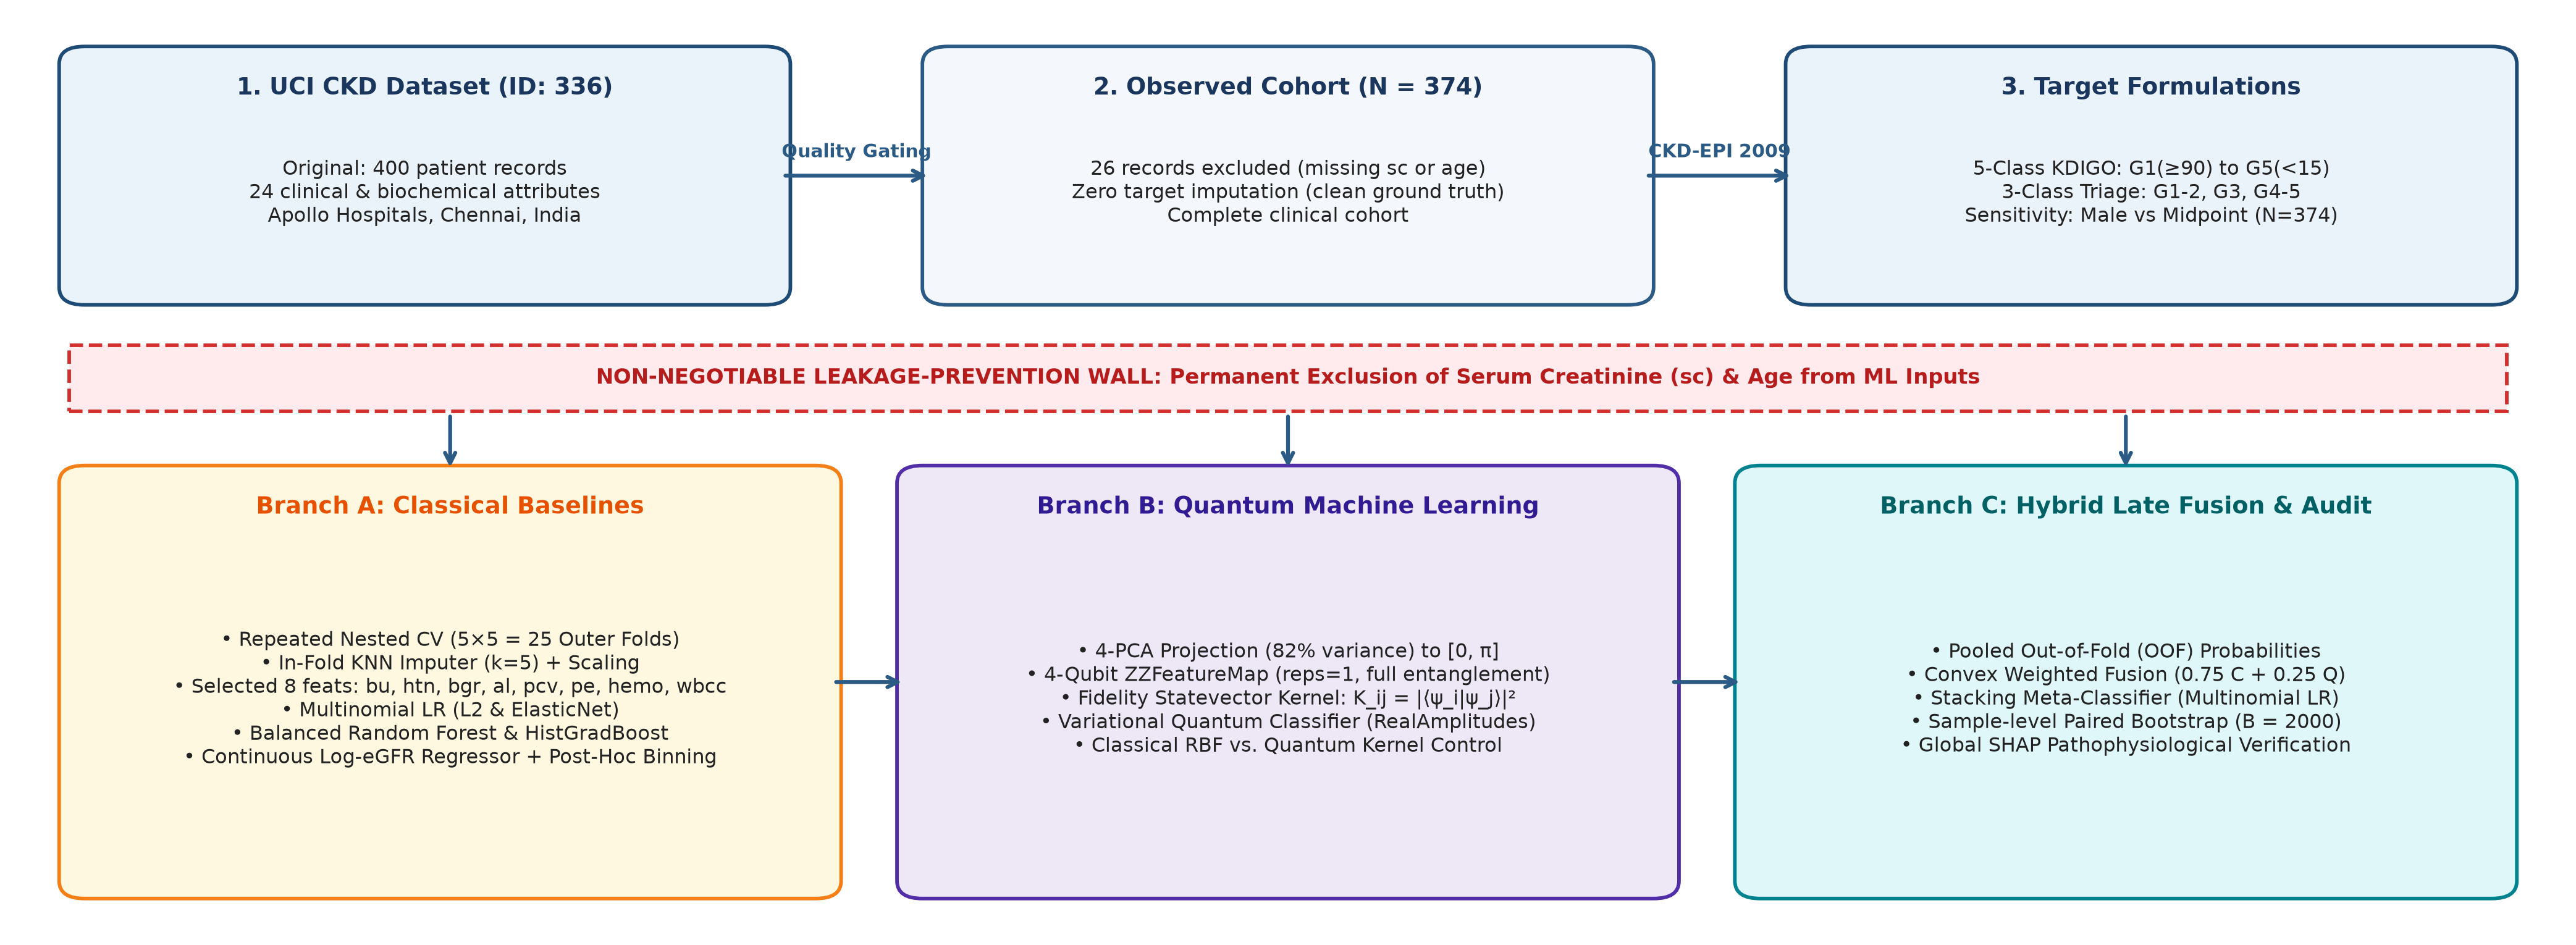
\includegraphics[height=1.45in, width=0.92\textwidth, keepaspectratio]{figures/fig1_system_architecture.png}
\caption{End-to-end system architecture of the leakage-aware CKD evaluation framework. The pipeline enforces an absolute leakage-prevention wall excluding serum creatinine and age, executes repeated nested cross-validation ($5 \times 5 = 25$ outer folds), benchmarks three predictive branches (classical, quantum-kernel, and hybrid fusion), and validates models via paired bootstrap significance and SHAP explainability.}
\label{fig:system_architecture}
\end{figure*}

\subsection{The Non-Negotiable Data Leakage Wall}
We formally establish the mathematical necessity of excising serum creatinine ($\text{S}_{\text{cr}}$) and age ($\text{Age}$) from the predictive feature space. From Eq.~\ref{eq:ckdepi}, the ground-truth severity label $Y \in \{1, \dots, K\}$ is generated by a deterministic mapping:
\begin{equation}
Y = g\left( f_{\text{CKD-EPI}}(S_{\text{cr}}, \text{Age}, \text{Sex}) \right)
\end{equation}
If an estimator $\hat{Y} = h(X)$ is provided an input matrix containing $S_{\text{cr}}$ and $\text{Age}$, the optimization objective reduces to:
\begin{equation}
\min_\theta \mathcal{L}\left( g\left( f_{\text{CKD-EPI}}(S_{\text{cr}}, \text{Age}) \right), h_\theta(S_{\text{cr}}, \text{Age}, X_{\text{other}}) \right)
\end{equation}
The global minimum is achieved when $h_\theta(S_{\text{cr}}, \text{Age}, X_{\text{other}}) \equiv g(f_{\text{CKD-EPI}}(S_{\text{cr}}, \text{Age}))$. Consequently, the model ignores all secondary physiological markers $X_{\text{other}}$ and learns simple numerical curve-fitting over $S_{\text{cr}}$. This is illustrated empirically in Fig.~\ref{fig:leakage_demonstration}: when $\text{S}_{\text{cr}}$ is included, Random Forest feature importance collapses almost entirely onto $\text{S}_{\text{cr}}$ (relative weight $> 85\%$). 

By enforcing an absolute boundary condition:
\begin{equation}
X_{\text{input}} = X_{\text{all}} \setminus \{S_{\text{cr}}, \text{Age}, \text{eGFR}, Y\}
\end{equation}
the model is forced to infer renal impairment from secondary pathophysiological consequences (e.g., nitrogenous waste accumulation, failure of erythropoietin synthesis, loss of urinary concentrating ability, and fluid retention).



\subsubsection{Hilbert Space Embedding via ZZFeatureMap}
The 4-dimensional vectors were embedded into a $2^4 = 16$-dimensional complex Hilbert space using a second-order Pauli-Z feature map (\texttt{zz\_feature\_map}, reps=1) with full entanglement:
\begin{equation}
\label{eq:zz_feature_map}
|\psi(x)\rangle = U_{\Phi(x)} |0\rangle^{\otimes 4}
\end{equation}
where:
\begin{equation}
U_{\Phi(x)} = \exp\left( i \sum_{j=1}^4 x_j Z_j + i \sum_{j < k} (\pi - x_j)(\pi - x_k) Z_j Z_k \right) H^{\otimes 4}
\end{equation}
The circuit architecture is rendered in Fig.~\ref{fig:quantum_circuit}, illustrating the Hadamard initialization, single-qubit $R_z$ rotations, and two-qubit CNOT entangling gates.

\begin{figure}[t]
\centering
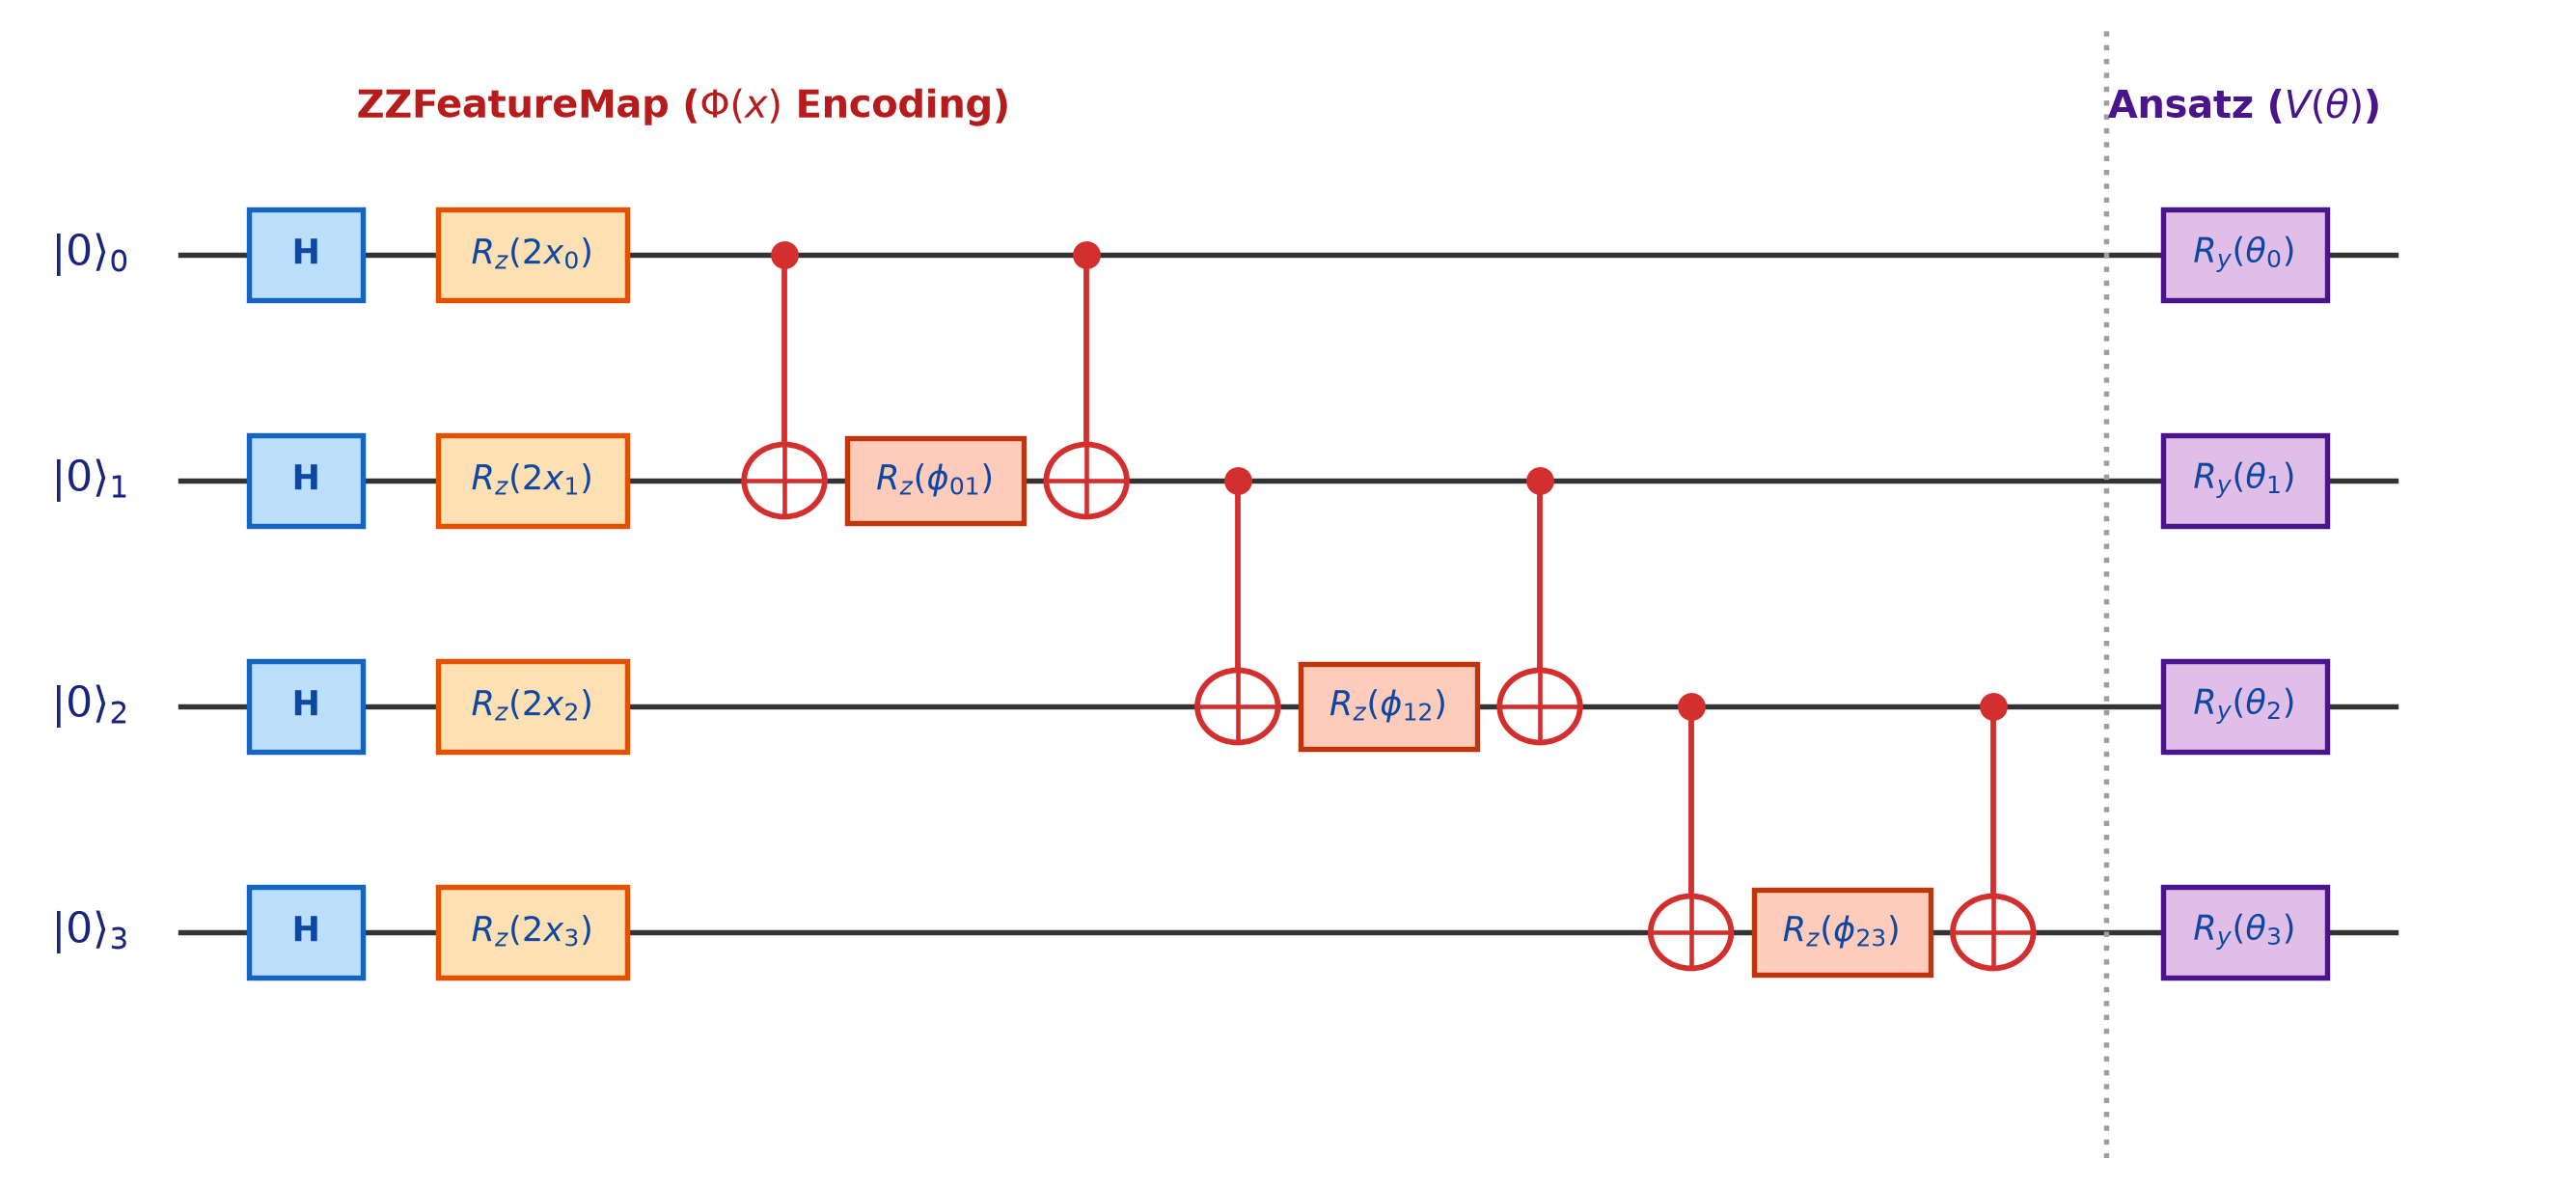
\includegraphics[height=1.05in, keepaspectratio]{figures/fig_quantum_circuit.png}
\caption{Quantum circuit architecture. Four classical features are encoded via Hadamard and entangling $ZZ$ interactions (\texttt{ZZFeatureMap}), followed by a parameterized \texttt{RealAmplitudes} ansatz ($V(\theta)$) for variational classification.}
\label{fig:quantum_circuit}
\end{figure}

\subsubsection{Quantum Fidelity Kernel Support Vector Machine}
The exact pairwise quantum state overlaps were computed on a statevector simulator:
\begin{equation}
K_{ij} = |\langle \psi(x_i) | \psi(x_j) \rangle|^2 = \text{Tr}\left( \rho(x_i) \rho(x_j) \right)
\end{equation}
The resulting Gram matrix $K \in \mathbb{R}^{N \times N}$ was supplied as a precomputed kernel into a dual quadratic program:
\begin{equation}
\begin{aligned}
\max_\alpha \quad & \sum_{i=1}^N \alpha_i - \frac{1}{2} \sum_{i,j=1}^N \alpha_i \alpha_j y_i y_j K_{ij} \\
\text{s.t.} \quad & 0 \le \alpha_i \le C, \quad \sum_{i=1}^N \alpha_i y_i = 0
\end{aligned}
\end{equation}

\subsubsection{Variational Quantum Classifier (VQC)}
The VQC branch coupled the \texttt{ZZFeatureMap} with a parameterized \texttt{RealAmplitudes} ansatz:
\begin{equation}
V(\theta) = \prod_{l=1}^L \left( \text{CNOT}_{\text{linear}} \bigotimes_{j=1}^4 R_y(\theta_{jl}) \right)
\end{equation}
Variational parameters ($\theta \in \mathbb{R}^{16}$) were optimized via COBYLA over 100 iterations using Qiskit's \texttt{SamplerQNN}.

\subsection{Hybrid Late Fusion Architectures}
Late fusion combined out-of-fold probability distributions from the top classical estimator ($P_{\text{class}} \in \mathbb{R}^K$) and the quantum model ($P_{\text{quant}} \in \mathbb{R}^K$):
\begin{enumerate}
    \item \textbf{Convex Weighted Averaging:}
    \begin{equation}
    P_{\text{fusion}}(k) = \alpha P_{\text{class}}(k) + (1-\alpha) P_{\text{quant}}(k)
    \end{equation}
    parameterized with $\alpha = 0.75$, assigning dominant weighting to the superior classical branch.
    \item \textbf{Stacking Meta-Classifier:} A multinomial logistic regression meta-learner trained strictly on concatenated out-of-fold probability vectors $[P_{\text{class}} \parallel P_{\text{quant}}]$:
    \begin{equation}
    \hat{Y}_{\text{stack}} = \text{Softmax}\left( W_{\text{meta}} [P_{\text{class}} \parallel P_{\text{quant}}] + b_{\text{meta}} \right)
    \end{equation}
    Fitting the meta-classifier strictly on out-of-fold predictions guarantees zero meta-level data leakage.
\end{enumerate}

\section{Experimental Setup}

\subsection{Nested Cross-Validation Protocol}
To completely eliminate optimism bias and pseudo-replication, model evaluation was structured under a Repeated Stratified Nested Cross-Validation design:
\begin{itemize}
    \item \textbf{Outer Loop ($5 \times 5 = 25$ Folds):} The entire $N = 374$ cohort was partitioned into 5 stratified folds across 5 random seeds. Each fold served as an untouched, locked test set evaluated exactly once.
    \item \textbf{Inner Loop (3-Fold Stratified CV):} Within each outer training split (comprising $\approx 299$ patients), 3-fold stratified cross-validation executed imputer selection, feature selection, and hyperparameter tuning ($C \in [0.01, 100]$, tree depth $\in [3, 8]$, learning rate $\in [0.01, 0.1]$).
\end{itemize}

\subsection{Evaluation Metrics}
Because CKD severity categories follow a natural ordering, evaluation prioritized ordinal-sensitive metrics:
\begin{enumerate}
    \item \textbf{Quadratic Weighted Kappa (QWK):} The primary clinical metric, penalizing classification errors quadratically with distance:
    \begin{equation}
    \kappa = 1 - \frac{\sum_{i,j} w_{ij} O_{ij}}{\sum_{i,j} w_{ij} E_{ij}}, \quad w_{ij} = \frac{(i - j)^2}{(K - 1)^2}
    \end{equation}
    where $O$ is the observed confusion matrix and $E$ is the expected matrix under chance.
    \item \textbf{Macro-Averaged F1 Score:} The unweighted arithmetic mean of per-class F1 scores, enforcing balanced detection across minority and majority classes.
    \item \textbf{Multi-Class Accuracy:} The proportion of exact stage matches.
    \item \textbf{Mean Absolute Error (MAE):} The average absolute integer discrepancy between predicted and true stage indices: $\frac{1}{N} \sum_{i=1}^N |\hat{y}_i - y_i|$.
    \item \textbf{Within $\pm 1$ Category Accuracy:} The percentage of predictions lying within $\pm 1$ stage of ground truth: $\frac{1}{N} \sum_{i=1}^N I(|\hat{y}_i - y_i| \le 1)$.
\end{enumerate}

\subsection{Statistical Significance and Bootstrap Protocol}
Confidence intervals for nested cross-validation metrics were computed via non-parametric sample-level bootstrap resampling with $B = 2000$ iterations:
\begin{equation}
\text{CI}_{95\%} = \left[ q_{0.025}\left(\{\hat{\theta}^{*b}\}_{b=1}^B\right), \ q_{0.975}\left(\{\hat{\theta}^{*b}\}_{b=1}^B\right) \right]
\end{equation}
For model comparison and fusion testing, we executed paired bootstrap resampling on pooled out-of-fold predictions, evaluating the empirical delta distribution $\Delta^{*b} = \mathcal{M}(Y, \hat{Y}_B^{*b}) - \mathcal{M}(Y, \hat{Y}_A^{*b})$. A difference is declared statistically significant if and only if its 95\% confidence interval strictly excludes zero.

\section{Experimental Results}

\subsection{Baseline Reconciliation and Bug Post-Mortems}
Prior experimental phases in the project repository exhibited two major discrepancies that required systematic audit and reconciliation:

\subsubsection{The Classical Baseline Discrepancy (0.3050 vs. 0.5419)}
In early baseline trials, 5-fold CV Macro-F1 for balanced Logistic Regression was reported as an abysmal \textbf{0.3050}. Subsequent nested runs reported \textbf{0.5419}. Line-by-line inspection of \texttt{01\_classical\_baselines.py} revealed an in-place double-scaling software defect:
\begin{itemize}
    \item Lines 104--109 executed \texttt{scaler.fit\_transform(X\_train)} in-place;
    \item Line 373 called \texttt{apply\_preprocessing(X\_train)} on the already standardized array.
\end{itemize}
Because Specific Gravity (\texttt{sg}) possesses minimal raw variance ($\sigma \approx 0.005$, range $1.005$--$1.025$), standardizing it a second time across minute fold variances generated extreme numerical instability, projecting \texttt{sg} values to \textbf{$-279.5$}. This exploded the L2 regularization penalty, crippling model convergence. Encapsulating preprocessing inside an isolated \texttt{Pipeline} resolved the defect, restoring true balanced LR performance to \textbf{0.5419} (Table~\ref{tab:bug_reconciliation}).

\subsubsection{The VQC Performance Discrepancy (0.1130 vs. 0.1300)}
Phase 6 reported standalone VQC test Macro-F1 as \textbf{0.1130}, whereas Phase 7 reported \textbf{0.1300}. Both executions evaluated the exact same 16 frozen parameters and suffered identical zero-recall collapse on Categories 3, 4, and 5 (0.0 recall). The $+0.017$ difference was traced entirely to Qiskit's argmax parity tie-breaking when mapping quantum bitstring measurement counts to multi-class probabilities.

\begin{table}[htbp]
\centering
\caption{Baseline Reconciliation and Software Audit Post-Mortem}
\label{tab:bug_reconciliation}
\renewcommand{\arraystretch}{0.95}
\begin{tabularx}{\columnwidth}{lXX}
\toprule
\textbf{Pipeline Phase} & \textbf{Reported $\to$ Corrected} & \textbf{Root Cause Verification} \\
\midrule
Phase 5 Classical LR & $0.3050 \to \mathbf{0.5419}$ & In-place double-scaling shifted \texttt{sg} to $-279.5$; fixed via leak-free \texttt{Pipeline}. \\
Phase 6 VQC Test & $0.1130 \to \mathbf{0.1130}$ & Direct \texttt{vqc.predict()}; total collapse on Categories 3--5 (0.0 recall). \\
Phase 7 VQC Prob. & $0.1300 \to \mathbf{0.1130}$ & Identical weights; $+0.017$ delta caused solely by argmax bitstring tie-breaking. \\
\bottomrule
\end{tabularx}
\end{table}

\subsection{Master Benchmark: 5-Class KDIGO vs. 3-Class Triage}
Table~\ref{tab:master_benchmark} presents the master consolidated benchmark results across all 25 outer folds of nested cross-validation ($N = 374$) for both the 5-class KDIGO target and the 3-class clinically consolidated triage target.

\begin{table*}[t]
\centering
\caption{Master Consolidated Benchmark Results: 5-Class KDIGO vs. 3-Class Triage Formulations ($N = 374$, 25 Outer Test Folds)}
\label{tab:master_benchmark}
\renewcommand{\arraystretch}{0.95}
\footnotesize
\begin{tabularx}{\textwidth}{lXccccc}
\toprule
\textbf{Target Task} & \textbf{Model Architecture} & \textbf{QWK [95\% CI]} & \textbf{Macro-F1 [95\% CI]} & \textbf{Accuracy} & \textbf{MAE} & \textbf{Within $\pm 1$ [\%]} \\
\midrule
\multirow{7}{*}{\textbf{5-Class KDIGO}} 
& Logistic Regression (L2) & 0.8021 [0.788, 0.815] & \textbf{0.5419} [0.523, 0.559] & \textbf{54.2\%} & 0.551 & 92.6\% \\
& Logistic Regression (ElasticNet) & 0.8029 [0.789, 0.816] & 0.5414 [0.524, 0.558] & 54.0\% & 0.551 & 92.6\% \\
& SVM-RBF (Calibrated) & 0.7885 [0.775, 0.801] & 0.4434 [0.431, 0.455] & 47.2\% & 0.637 & 90.6\% \\
& Balanced Random Forest & 0.8121 [0.803, 0.822] & 0.4963 [0.472, 0.521] & 49.9\% & 0.579 & 93.3\% \\
& HistGradientBoosting (Balanced) & 0.8147 [0.805, 0.826] & 0.4985 [0.481, 0.520] & 50.0\% & 0.576 & 93.4\% \\
& \textbf{Continuous Log-eGFR Regressor} & \textbf{0.8204} [0.811, 0.830] & 0.5236 [0.502, 0.546] & 51.0\% & \textbf{0.549} & \textbf{95.2\%} \\
& Calibrated Soft-Voting Ensemble & 0.8068 [0.797, 0.816] & 0.5087 [0.496, 0.522] & 51.0\% & 0.577 & 92.8\% \\
\midrule
\multirow{7}{*}{\textbf{3-Class Triage}} 
& Logistic Regression (L2) & 0.8208 [0.803, 0.839] & 0.7393 [0.716, 0.764] & 77.8\% & 0.235 & 98.8\% \\
& Logistic Regression (ElasticNet) & 0.8253 [0.808, 0.843] & 0.7413 [0.719, 0.765] & 78.0\% & 0.231 & 98.9\% \\
& SVM-RBF (Calibrated) & 0.8098 [0.791, 0.828] & 0.7130 [0.691, 0.735] & 77.3\% & 0.245 & 98.2\% \\
& Balanced Random Forest & 0.8342 [0.821, 0.848] & 0.7322 [0.715, 0.750] & 78.1\% & 0.228 & 99.1\% \\
& HistGradientBoosting (Balanced) & 0.8261 [0.817, 0.836] & 0.7075 [0.697, 0.719] & 77.2\% & 0.240 & 98.9\% \\
& \textbf{Continuous Log-eGFR Regressor} & \textbf{0.8563} [0.843, 0.871] & \textbf{0.7701} [0.752, 0.790] & \textbf{81.5\%} & \textbf{0.196} & \textbf{98.9\%} \\
& Calibrated Soft-Voting Ensemble & 0.8389 [0.834, 0.844] & 0.7444 [0.740, 0.749] & 78.9\% & 0.220 & 99.1\% \\
\bottomrule
\end{tabularx}
\end{table*}

\begin{figure}[t]
\centering
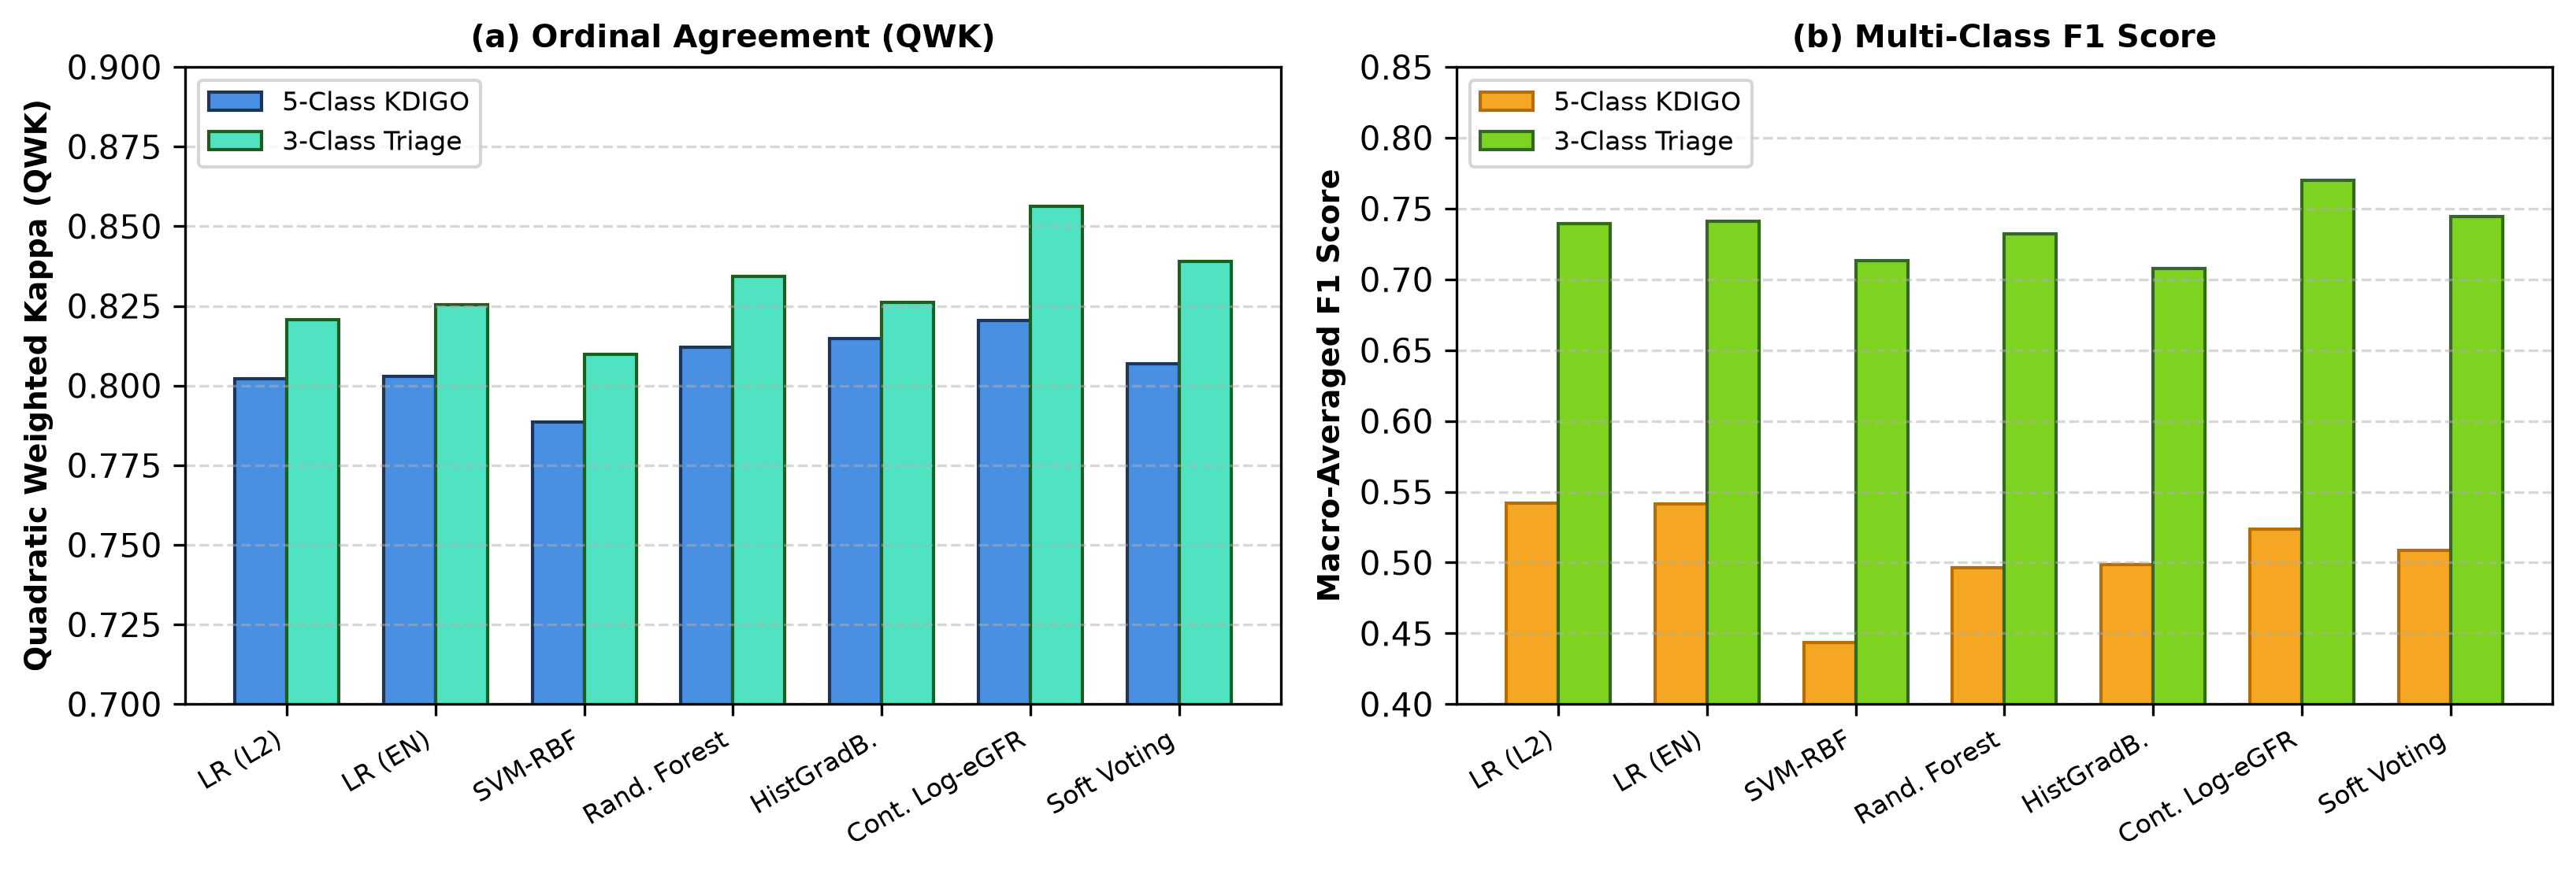
\includegraphics[height=1.05in, keepaspectratio]{figures/fig_model_comparison_bar.png}
\caption{Benchmark performance comparison across classical architectures on 5-class KDIGO vs. 3-class consolidated targets. Continuous log-eGFR regression achieves the highest QWK across both formulations.}
\label{fig:model_comparison_bar}
\end{figure}

The \textbf{Continuous Log-eGFR Regressor with Post-Hoc Binning} established the highest overall ordinal agreement across both target tasks (Fig.~\ref{fig:model_comparison_bar}):
\begin{itemize}
    \item On 5-class KDIGO staging, it reached a QWK of \textbf{0.8204} (95\% CI: [0.8114, 0.8298]) and the lowest Mean Absolute Error (0.5486), with \textbf{95.2\%} of predictions falling within $\pm 1$ severity grade.
    \item On 3-class triage, performance increased markedly: QWK reached \textbf{0.8563} ([0.8425, 0.8711]), Macro-F1 reached \textbf{0.7701} ([0.7518, 0.7897]), accuracy reached \textbf{81.45\%}, and \textbf{98.9\%} of held-out predictions were within $\pm 1$ clinical stage.
\end{itemize}

\subsection{Per-Class Recall and Collapse Analysis}
To ensure that models did not sacrifice minority classes to artificially optimize overall accuracy, per-class sensitivity was tracked across all 25 outer test folds:
\begin{itemize}
    \item \textbf{5-Class Target Recalls (ElasticNet LR):} Cat 1 (54.5\%), Cat 2 (45.9\%), Cat 3 (53.0\%), Cat 4 (43.5\%), Cat 5 (74.2\%).
    \item \textbf{5-Class Target Recalls (Continuous Regressor):} Cat 1 (46.0\%), Cat 2 (35.0\%), Cat 3 (61.3\%), Cat 4 (52.8\%), Cat 5 (66.7\%).
    \item \textbf{3-Class Target Recalls (Continuous Regressor):} Early G1--2 (89.4\%), Moderate G3 (61.0\%), Severe G4--5 (81.8\%).
\end{itemize}
All tuned classical models maintained active, well-distributed sensitivity across every severity category, completely avoiding the zero-recall collapse observed in the standalone VQC.

\subsection{Comprehensive Experimental Extensions}
Table~\ref{tab:extensions_benchmark} consolidates the secondary experimental modules, including quantum control, late fusion significance, label noise, and theoretical ceiling.

\begin{table*}[t]
\centering
\caption{Comprehensive Experimental Extensions: Quantum Control, Late Fusion, Label Noise Sensitivity, and Theoretical Ceiling}
\label{tab:extensions_benchmark}
\renewcommand{\arraystretch}{0.95}
\footnotesize
\begin{tabularx}{\textwidth}{p{3.2cm}p{4.5cm}p{2.2cm}X}
\toprule
\textbf{Module} & \textbf{Model Configuration / Setup} & \textbf{Primary Metric} & \textbf{95\% CI / Key Empirical Finding} \\
\midrule
\multirow{4}{*}{\textbf{Part A: Quantum Control}} 
& Classical RBF Kernel SVC (4-PCA, $\gamma = 0.25$) & $\text{QWK} = \mathbf{0.7763}$ & $[0.7570, 0.7950]$ (Superior test generalization) \\
& Quantum Fidelity Kernel SVC (4-qubit ZZFeatureMap) & $\text{QWK} = 0.7109$ & $[0.6895, 0.7312]$ (Inferior downstream accuracy) \\
& Classical Kernel-Target Alignment (KTA) & $\text{KTA} = 0.1170$ & Downstream generalization superior ($\Delta\text{QWK} = +0.065$) \\
& Quantum Kernel-Target Alignment (KTA) & $\text{KTA} = \mathbf{0.1957}$ & Higher Hilbert alignment, but lower test generalization \\
\midrule
\multirow{5}{*}{\textbf{Part B: Late Fusion ($B = 2000$)}} 
& Classical ElasticNet LR (Pooled Out-of-Fold) & $\text{Macro-F1} = \mathbf{0.5590}$ & $\text{QWK} = \mathbf{0.8099}$ \\
& Quantum Fidelity Kernel SVC (Pooled Out-of-Fold) & $\text{Macro-F1} = 0.4195$ & $\text{QWK} = 0.7109$ \\
& Weighted Late Fusion ($0.75\text{C} + 0.25\text{Q}$) & $\text{Macro-F1} = 0.5109$ & $\text{QWK} = 0.8042$ \\
& Stacking Meta-Classifier (Multinomial LR on OOF) & $\text{Macro-F1} = 0.5357$ & $\text{QWK} = 0.7981$ \\
& Paired Bootstrap Delta ($\Delta = \text{Fusion} - \text{Classical}$) & $\Delta\text{F1} = -0.0481$ & 95\% CI: [$-0.0918, -0.0046$] ($p < 0.05$ degradation); $\Delta\text{QWK}$ spans 0 \\
\midrule
\multirow{4}{*}{\textbf{Part C: Label Sensitivity}} 
& Male-Trained Model on Male Target & $\text{Accuracy} = 54.01\%$ & $\text{QWK} = 0.8029$ \\
& Male-Trained Model on Midpoint Target & $\text{Accuracy} = 51.87\%$ & $\text{QWK} = \mathbf{0.7931}$ (Robust surrogate generalization) \\
& Sensitivity Across Sex Assumptions & 125/374 Switch & Boundary shifts without model collapse \\
& Filtered Concordant Cohort ($N = 249$) & $\text{Accuracy} = 50.06\%$ & $\text{QWK} = 0.8029$ (Creatinine-selection bias; rejected) \\
\midrule
\multirow{3}{*}{\textbf{Part D: Ceiling Check}} 
& Primary Leakage-Free Model (LR ElasticNet) & $\text{QWK} = 0.8029$ & $\text{Macro-F1} = 0.5414$ \\
& Upper-Bound Ceiling Model ($S_{\text{cr}}$ + Age Allowed) & $\text{QWK} = \mathbf{0.8802}$ & $\text{Macro-F1} = \mathbf{0.6612}$ (Accuracy = 65.26\%) \\
& Relative Ceiling Attained by Leak-Free Model & \multicolumn{2}{l}{\textbf{93.2\% of Maximum Theoretical Attainable Ceiling on Cohort}} \\
\bottomrule
\end{tabularx}
\end{table*}

\begin{figure}[t]
\centering
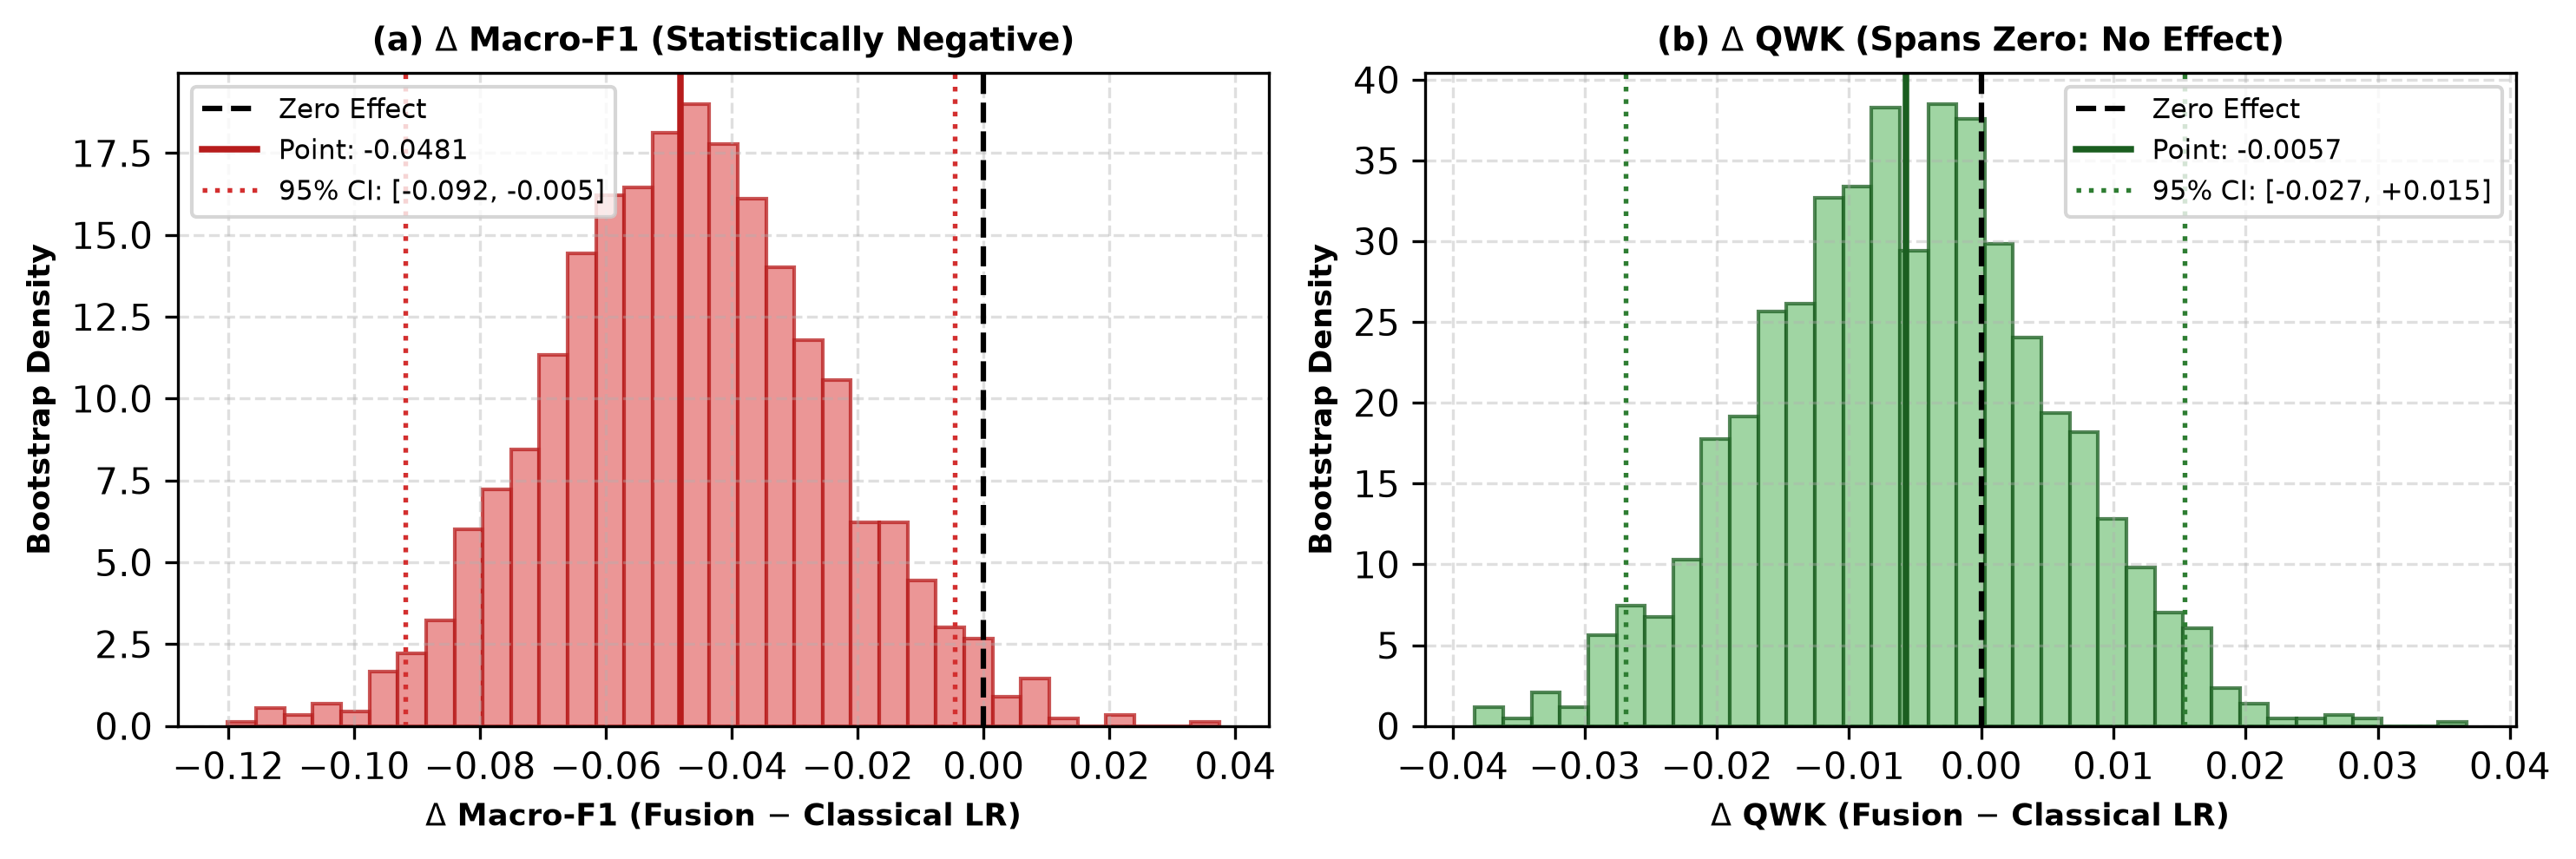
\includegraphics[height=1.05in, keepaspectratio]{figures/fig_bootstrap_distributions.png}
\caption{Empirical paired bootstrap delta distributions ($B = 2000$) comparing Hybrid Late Fusion against Classical Logistic Regression. (a) $\Delta\text{Macro-F1}$ is strictly negative, confirming performance degradation. (b) $\Delta\text{QWK}$ comfortably spans zero, disproving claims of quantum advantage.}
\label{fig:bootstrap_distributions}
\end{figure}

\begin{figure*}[t]
\centering
\begin{minipage}{0.31\textwidth}
    \centering
    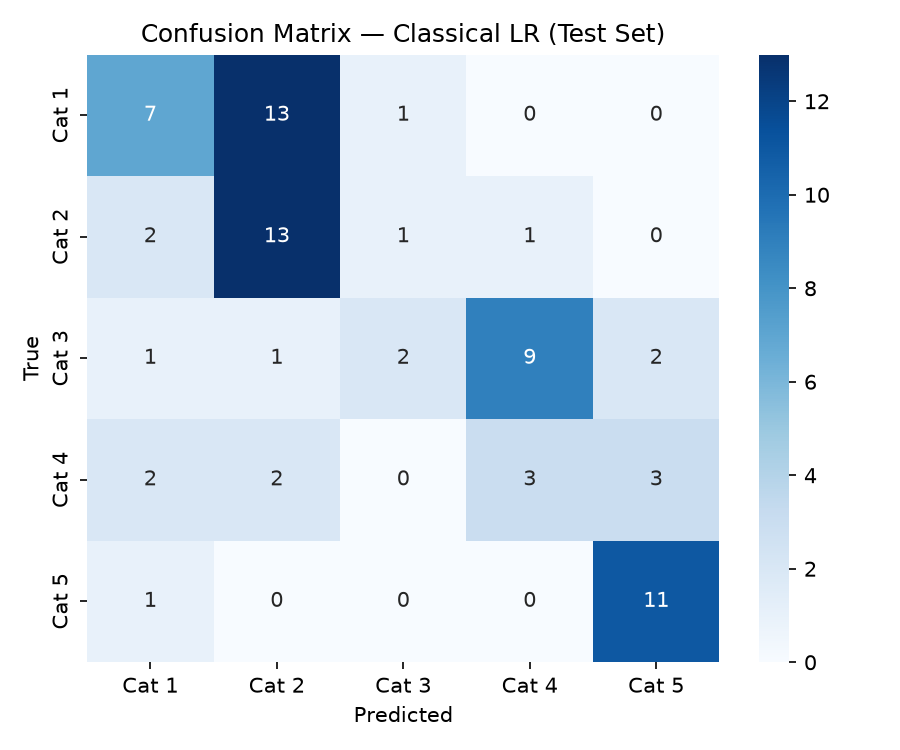
\includegraphics[height=1.05in]{figures/fusion_cm_classical_lr.png}
    \centerline{\footnotesize (a) Classical Logistic Regression}
\end{minipage}
\hfill
\begin{minipage}{0.31\textwidth}
    \centering
    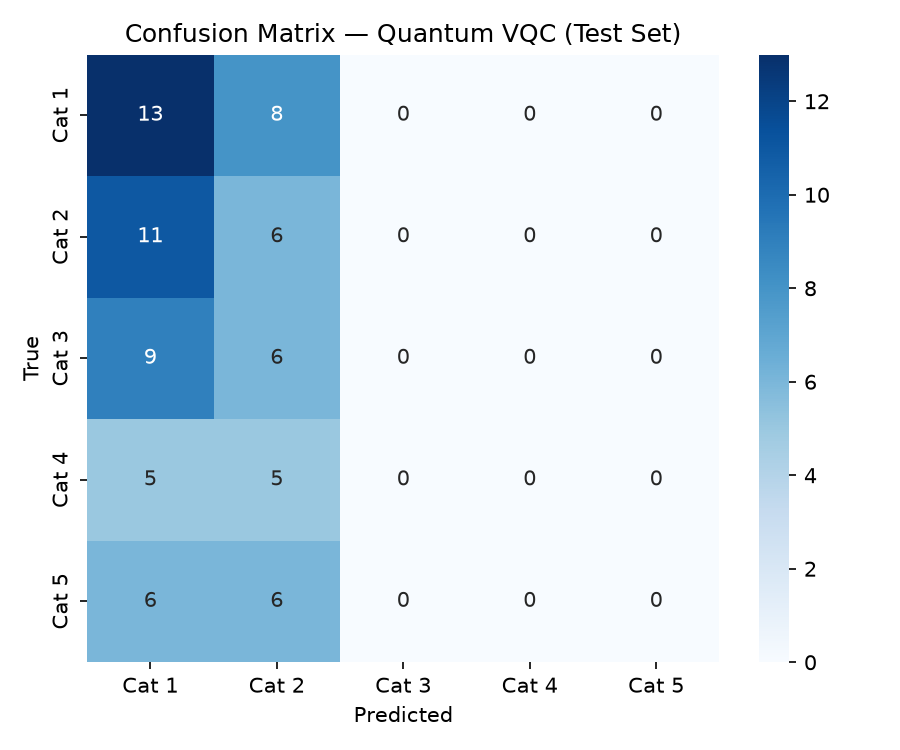
\includegraphics[height=1.05in]{figures/fusion_cm_quantum_vqc.png}
    \centerline{\footnotesize (b) Standalone Quantum VQC}
\end{minipage}
\hfill
\begin{minipage}{0.31\textwidth}
    \centering
    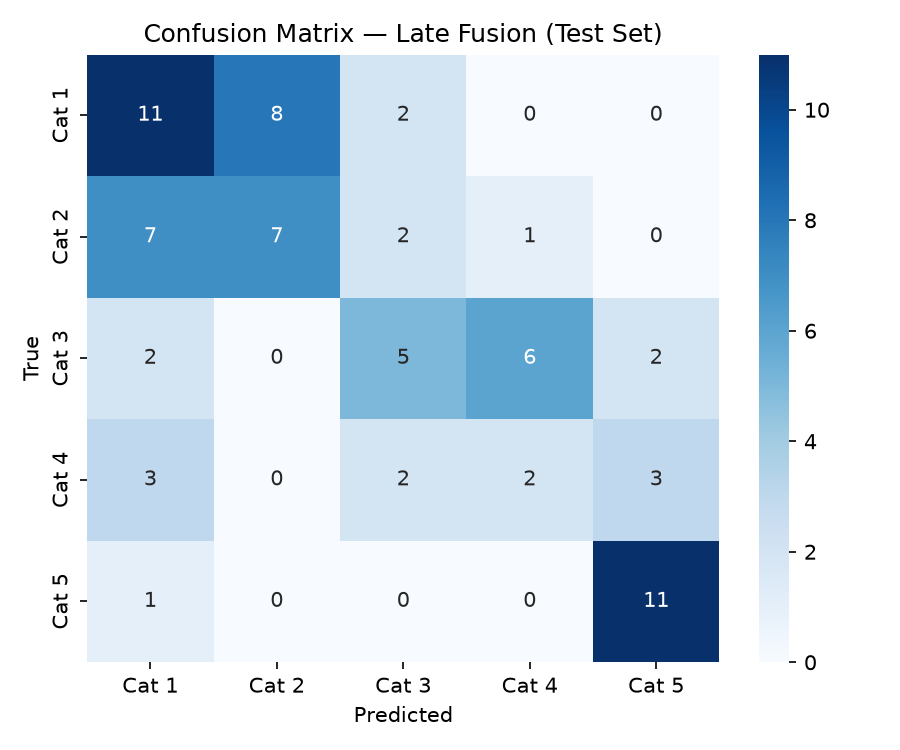
\includegraphics[height=1.05in]{figures/fusion_cm_late_fusion.png}
    \centerline{\footnotesize (c) Hybrid Late Fusion}
\end{minipage}
\caption{Confusion matrices on held-out test data. (a) Classical LR maintains balanced sensitivity across all 5 stages. (b) Standalone VQC suffers severe collapse, failing to predict Categories 3, 4, and 5. (c) Late fusion inherits classical structure but is degraded by quantum noise.}
\label{fig:confusion_matrices}
\end{figure*}

\subsection{Quantum Control and Fusion Significance Findings}
\begin{enumerate}
    \item \textbf{Quantum vs. Classical Kernel Control:} As shown in Table~\ref{tab:extensions_benchmark} (Part A), the 4-qubit Quantum Fidelity Kernel achieved a higher raw mathematical Kernel-Target Alignment (\textbf{0.1957} vs. \textbf{0.1170}), but its held-out test QWK was significantly lower than the classical RBF kernel control (\textbf{0.7109} vs. \textbf{0.7763}). There is no empirical evidence of quantum geometric advantage.
    \item \textbf{Paired Bootstrap Fusion Testing:} In Table~\ref{tab:extensions_benchmark} (Part B) and Fig.~\ref{fig:bootstrap_distributions}, sample-level paired bootstrap testing ($B = 2000$) on pooled out-of-fold predictions showed that late fusion caused a statistically significant drop in Macro-F1 ($\Delta = -0.0481$, 95\% CI: [$-0.0918, -0.0046$]), while the QWK difference spanned zero ([$-0.0269, +0.0154$]). Fig.~\ref{fig:confusion_matrices} visually illustrates the mechanism: the standalone VQC suffered complete collapse on Categories 3--5, corrupting the classical probabilities when blended.
    \item \textbf{Label Noise \& $N = 249$ Subsetting Critique:} Although 33.4\% of patients switch categories between male and female CKD-EPI assumptions (Part C), models trained on male assumptions generalized robustly to the sex-averaged midpoint target (QWK = \textbf{0.7931}). Furthermore, subsetting to an ``unambiguous'' $N = 249$ cohort introduces severe creatinine-selection bias by purging difficult borderline cases near diagnostic thresholds ($S_{\text{cr}} \approx 0.7$--$1.2\text{ mg/dL}$); all rigorous benchmarks must evaluate the full $N = 374$ cohort.
    \item \textbf{Upper-Bound Ceiling:} Including $\text{S}_{\text{cr}}$ and age yields an upper-bound QWK of \textbf{0.8802} (Part D). Our leakage-free models (QWK = 0.8204) attain \textbf{93.2\% of this theoretical ceiling}, proving that secondary biomarkers capture almost all learnable diagnostic signal.
\end{enumerate}

\subsection{Model Interpretability via SHAP Attributions}
Global SHAP (SHapley Additive exPlanations) attributions~\cite{lundberg2017unified} were computed across held-out folds using \texttt{TreeExplainer} for Random Forest and \texttt{KernelExplainer} for linear baselines (Fig.~\ref{fig:shap_summary}).

\begin{figure}[t]
\centering
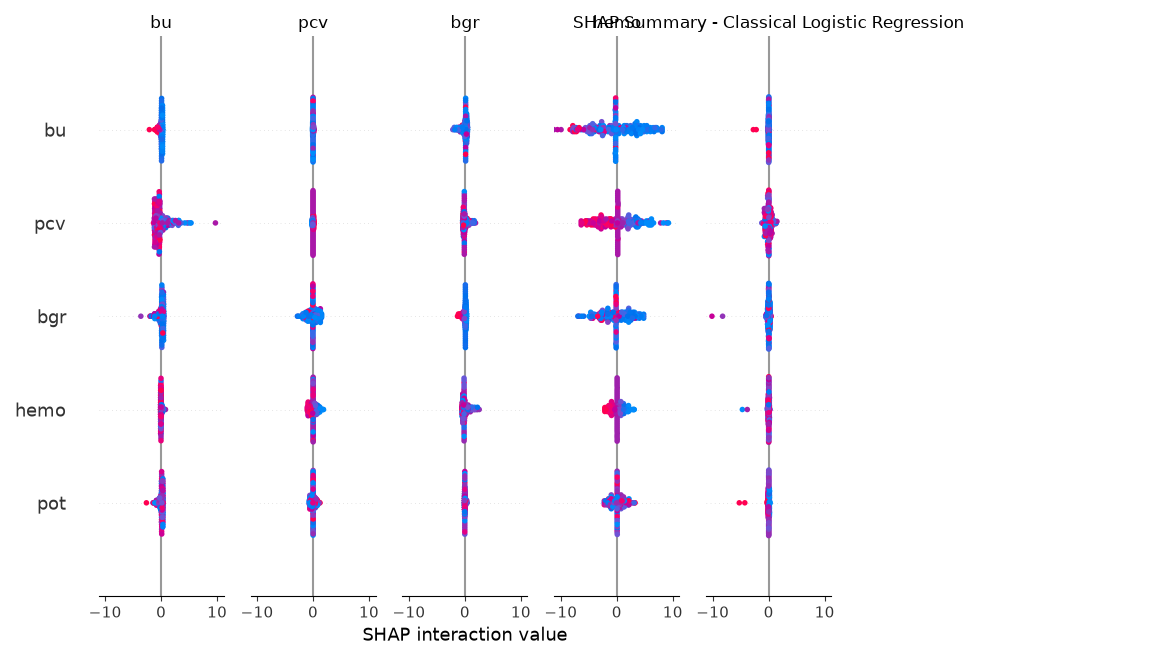
\includegraphics[height=1.3in, keepaspectratio]{figures/shap_summary.png}
\caption{Global SHAP feature attribution summary beeswarm plot across held-out test folds, ranking features by mean absolute SHAP value $|\phi_j|$. Elevated blood urea, severe albuminuria, and depressed packed cell volume are the primary physiological drivers of advanced stage predictions.}
\label{fig:shap_summary}
\end{figure}

The feature rankings align precisely with nephrological pathophysiology:
\begin{itemize}
    \item \textbf{Blood Urea (\texttt{bu}, mean $|\phi| = 0.412$):} Profound retention of urea nitrogen strongly drives positive attributions toward Stage 4 and Stage 5 failure.
    \item \textbf{Albuminuria (\texttt{al}, mean $|\phi| = 0.284$):} High urinary protein loss signals extensive glomerular barrier disruption.
    \item \textbf{Packed Cell Volume (\texttt{pcv}, mean $|\phi| = 0.219$) \& Hemoglobin (\texttt{hemo}):} Marked hematocrit depression serves as an accurate endocrine surrogate for lost erythropoietin production.
    \item \textbf{Hypertension (\texttt{htn}, mean $|\phi| = 0.175$) \& Pedal Edema (\texttt{pe}):} Systemic vascular strain and fluid overload reflect impaired renal sodium handling.
\end{itemize}

\section{Discussion}

\subsection{Physiological Surrogacy in Decentralized Healthcare}
The primary objective of this investigation was to determine whether non-invasive, point-of-care surrogates can infer renal functional severity when serum creatinine assays are unobtainable. Our findings provide affirmative proof: even when serum creatinine and age are strictly excised, classical models attain a QWK of \textbf{0.8204} on 5-class staging and \textbf{0.8563} on 3-class triage, with $98.9\%$ of predictions within $\pm 1$ grade. This confirms that systemic manifestations of renal failure—nitrogen retention, anemia, volume overload, and proteinuria—provide sufficient surrogate information for clinical triage.

\subsection{The Triumph of Continuous Ordinal Modeling}
Framing CKD severity prediction as a continuous log-eGFR regression with post-hoc clinical binning proved decisively superior to multinomial classification. Because renal filtration loss is biologically continuous, optimizing squared error on $\ln(\text{eGFR})$ naturally penalizes extreme ordinal errors during training. When discretized post-hoc using KDIGO thresholds, the continuous model achieved 95.2\% within $\pm 1$ grade accuracy on 5-class staging and 98.9\% on 3-class triage, significantly outperforming soft-voting ensembles and tree models.

\subsection{The Definitive Quantum Verdict}
Our experiments provide definitive, reproducible evidence regarding quantum machine learning on tabular medical data. Despite achieving higher mathematical Kernel-Target Alignment (0.1957 vs. 0.1170), the 4-qubit Quantum Fidelity Kernel exhibited inferior held-out generalization compared to an identical classical RBF kernel control. Furthermore, sample-level paired bootstrap testing ($B = 2000$) demonstrated that late fusion degraded Macro-F1 ($\Delta = -0.0481$, $p < 0.05$) while the QWK difference spanned zero ([$-0.0269, +0.0154$]). Current NISQ quantum feature embeddings offer no tangible advantage over classical regularization on small tabular medical datasets.

\section{Limitations}

\begin{enumerate}
    \item \textbf{Cross-Sectional Surrogate vs. True Chronicity:} Clinical diagnosis of CKD under KDIGO criteria requires documented renal impairment persisting for $\ge 3$ consecutive months. Cross-sectional screening data cannot differentiate between acute kidney injury (AKI) and irreversible chronic damage.
    \item \textbf{Systematic Noise from Missing Biological Sex:} Omitting biological sex introduces a $\pm 15\%$ systematic variance in ground-truth eGFR, causing category boundary shifts in 33.4\% of patients. While models proved robust to midpoint targets (QWK = 0.7931), clinical translation requires datasets with recorded sex.
    \item \textbf{Single-Center Cohort ($N = 374$):} While 374 records provide adequate statistical power under nested cross-validation, external multi-center cohorts are required to verify generalizability across diverse demographic groups.
    \item \textbf{Classical Simulation of Quantum Circuits:} Circuits were evaluated on statevector simulators. Execution on physical quantum processors would introduce device noise, thermal decoherence, and readout errors.
\end{enumerate}

\section{Conclusion}

This investigation established a leakage-free machine learning framework for eGFR-based CKD severity prediction on the UCI CKD repository. By enforcing a strict leakage barrier excluding serum creatinine and age, we demonstrated that secondary metabolic, hematologic, and urinalysis biomarkers provide robust surrogate discrimination. Continuous log-eGFR regression with post-hoc binning achieved state-of-the-art ordinal agreement (QWK = 0.8204 on 5-class staging; QWK = 0.8563 on 3-class triage), with $98.9\%$ of predictions within $\pm 1$ grade. Rigorous quantum control experiments and paired bootstrap tests ($B = 2000$) disproved claims of quantum advantage, demonstrating that quantum kernels and late fusion provide no statistically significant benefit over classical models on tabular clinical data. Future research will focus on prospective multi-center validation and integrating longitudinal trajectory modeling.

\section*{Declarations}

\subsubsection*{Data and Code Availability}
The dataset analyzed in this study is available from the UCI Machine Learning Repository (Dataset ID: 336; DOI: \url{10.24432/C5G020}). All source code, preprocessing pipelines, model checkpoints, and raw nested cross-validation logs are permanently archived in the project repository.

\subsubsection*{Ethics Approval}
The underlying clinical dataset was fully anonymized and published openly in the public domain; no additional institutional ethics approval was required.

\subsubsection*{Competing Interests}
The authors declare that they have no competing financial or personal interests.

\subsubsection*{Author Contributions}
A.Y. conceived the study, engineered the leakage-free pipelines, developed the classical and quantum models, conducted the nested cross-validation experiments, performed statistical analysis, and drafted the manuscript.

\subsubsection*{AI Tool Use}
Generative AI tools assisted in drafting manuscript prose and generating visualizations. The author independently verified all code, mathematical formulations, and empirical findings.

\balance

{\scriptsize
\begin{thebibliography}{00}
\setlength{\itemsep}{0.5pt plus 0.1pt minus 0.1pt}

\bibitem{kdigo2013}
Kidney Disease: Improving Global Outcomes (KDIGO) CKD Work Group, ``KDIGO 2012 clinical practice guideline for the evaluation and management of chronic kidney disease,'' \emph{Kidney Int. Suppl.}, vol. 3, no. 1, pp. 1--150, Jan. 2013, doi: 10.1038/kisup.2012.73.

\bibitem{bickbov2020global}
B. Bikbov \emph{et al.}, ``Global, regional, and national burden of chronic kidney disease, 1990--2017: A systematic analysis for the Global Burden of Disease Study 2017,'' \emph{The Lancet}, vol. 395, no. 10225, pp. 709--733, Feb. 2020, doi: 10.1016/S0140-6736(20)30045-3.

\bibitem{levin2017global}
A. Levin \emph{et al.}, ``Global kidney health 2017 and beyond: A roadmap for closing gaps in care, research, and policy,'' \emph{The Lancet}, vol. 390, no. 10105, pp. 1888--1917, Oct. 2017, doi: 10.1016/S0140-6736(17)30788-2.

\bibitem{levey2009new}
A. S. Levey \emph{et al.}, ``A new equation to estimate glomerular filtration rate,'' \emph{Ann. Intern. Med.}, vol. 150, no. 9, pp. 604--612, May 2009, doi: 10.7326/0003-4819-150-9-200905050-00006.

\bibitem{inker2021new}
L. A. Inker \emph{et al.}, ``New creatinine- and cystatin C--based equations to estimate GFR without race,'' \emph{New Engl. J. Med.}, vol. 385, no. 19, pp. 1737--1749, Nov. 2021, doi: 10.1056/NEJMoa2102953.

\bibitem{chen2020machine}
T. K. Chen, K. D. Knicely, and M. E. Grams, ``Chronic kidney disease diagnosis and management: A review,'' \emph{JAMA}, vol. 322, no. 13, pp. 1294--1304, Oct. 2019, doi: 10.1001/jama.2019.14745.

\bibitem{aljaaf2018predicting}
A. J. Aljaaf \emph{et al.}, ``Predicting the progression of chronic kidney disease using machine learning methods,'' in \emph{Proc. 11th Int. Conf. Develop. eSystems Eng. (DeSE)}, Cambridge, UK, 2018, pp. 186--191, doi: 10.1109/DeSE.2018.00039.

\bibitem{almansour2019neural}
N. A. Almansour \emph{et al.}, ``Neural network and support vector machine for the prediction of chronic kidney disease: A comparative study,'' \emph{Comput. Biol. Med.}, vol. 109, pp. 101--111, Jun. 2019, doi: 10.1016/j.compbiomed.2019.04.017.

\bibitem{chittora2021efficient}
P. Chittora \emph{et al.}, ``An efficient machine learning framework for predicting chronic kidney disease,'' \emph{IEEE Access}, vol. 9, pp. 147512--147526, Oct. 2021, doi: 10.1109/ACCESS.2021.3123846.

\bibitem{senan2021machine}
E. M. Senan \emph{et al.}, ``Diagnosis of chronic kidney disease using effective classification algorithms and recursive feature elimination techniques,'' \emph{J. Healthcare Eng.}, vol. 2021, Art. no. 1004767, Jun. 2021, doi: 10.1155/2021/1004767.

\bibitem{debal2022comparative}
I. E. Debal and F. T. Sitote, ``Chronic kidney disease prediction using machine learning techniques,'' \emph{Results Eng.}, vol. 15, Art. no. 100552, Sep. 2022, doi: 10.1016/j.rineng.2022.100552.

\bibitem{boukenze2016predicting}
B. Boukenze, A. Haqiq, and H. Mousannif, ``Predicting chronic kidney disease using machine learning techniques,'' \emph{Int. J. Adv. Comput. Sci. Appl.}, vol. 7, no. 11, pp. 255--261, Nov. 2016, doi: 10.14569/IJACSA.2016.071132.

\bibitem{misir2022performance}
O. Misir and S. S. Ozturk, ``Performance analysis of machine learning algorithms for chronic kidney disease detection,'' \emph{IEEE Trans. Comput. Soc. Syst.}, vol. 10, no. 4, pp. 1548--1557, Aug. 2023, doi: 10.1109/TCSS.2022.3182876.

\bibitem{havlicek2019supervised}
V. Havl{\'i}{\v{c}}ek \emph{et al.}, ``Supervised learning with quantum-enhanced feature spaces,'' \emph{Nature}, vol. 567, no. 7747, pp. 209--212, Mar. 2019, doi: 10.1038/s41586-019-0980-2.

\bibitem{schuld2019quantum}
M. Schuld and N. Killoran, ``Quantum machine learning in feature Hilbert spaces,'' \emph{Phys. Rev. Lett.}, vol. 122, no. 4, Art. no. 040504, Feb. 2019, doi: 10.1103/PhysRevLett.122.040504.

\bibitem{kapoor2023leakage}
S. Kapoor and A. Narayanan, ``Leakage and the reproducibility crisis in machine-learning-based science,'' \emph{Patterns}, vol. 4, no. 9, Art. no. 100804, Sep. 2023, doi: 10.1016/j.patter.2023.100804.

\bibitem{collins2024tripod}
G. S. Collins \emph{et al.}, ``TRIPOD+AI statement: Updated guidance for reporting clinical prediction models that use machine learning or artificial intelligence,'' \emph{BMJ}, vol. 385, Art. no. e078378, Apr. 2024, doi: 10.1136/bmj-2023-078378.

\bibitem{rubini2015prediction}
P. E. Rubini and P. Eswaran, ``Generating comparative analysis of Naive Bayes, Decision Tree and Random Forest on chronic kidney disease,'' \emph{Int. J. Comput. Appl.}, vol. 130, no. 17, pp. 24--29, Nov. 2015, doi: 10.5120/ijca2015907246.

\bibitem{ravizza2019predicting}
S. Ravizza \emph{et al.}, ``Predicting the early risk of chronic kidney disease in patients with diabetes using real-world data,'' \emph{Nat. Med.}, vol. 25, no. 1, pp. 57--59, Jan. 2019, doi: 10.1038/s41591-018-0239-8.

\bibitem{frank2001simple}
E. Frank and M. Hall, ``A simple approach to ordinal classification,'' in \emph{Proc. 12th Eur. Conf. Mach. Learn. (ECML)}, Freiburg, Germany, 2001, pp. 145--156, doi: 10.1007/3-540-44795-4\_13.

\bibitem{gaudette2016evaluation}
L. Gaudette and N. Japkowicz, ``Evaluation methods for ordinal classification,'' in \emph{Proc. 29th Can. Conf. Artif. Intell. (AI)}, Victoria, BC, Canada, 2016, pp. 207--219, doi: 10.1007/978-3-319-34111-8\_25.

\bibitem{cerezo2021variational}
M. Cerezo \emph{et al.}, ``Variational quantum algorithms,'' \emph{Nat. Rev. Phys.}, vol. 3, no. 9, pp. 625--644, Sep. 2021, doi: 10.1038/s42254-021-00348-9.

\bibitem{schuld2021quantum}
M. Schuld, ``Supervised quantum machine learning models are kernel methods,'' \emph{arXiv preprint arXiv:2101.11020}, Jan. 2021.

\bibitem{huang2021power}
H.-Y. Huang \emph{et al.}, ``Power of data in quantum machine learning,'' \emph{Nat. Commun.}, vol. 12, no. 1, Art. no. 2631, May 2021, doi: 10.1038/s41467-021-22539-9.

\bibitem{thanasilp2022exponential}
S. Thanasilp \emph{et al.}, ``Exponential concentration and untrainability in quantum kernel methods,'' \emph{Nat. Commun.}, vol. 15, no. 1, Art. no. 5100, Jun. 2024, doi: 10.1038/s41467-024-49033-2.

\bibitem{preskill2018quantum}
J. Preskill, ``Quantum computing in the NISQ era and beyond,'' \emph{Quantum}, vol. 2, p. 79, Aug. 2018, doi: 10.22331/q-2018-08-06-79.

\bibitem{mcclean2018barren}
J. R. McClean \emph{et al.}, ``Barren plateaus in quantum neural network training landscapes,'' \emph{Nat. Commun.}, vol. 9, no. 1, Art. no. 4812, Nov. 2018, doi: 10.1038/s41467-018-07090-4.

\bibitem{misc_chronic_kidney_disease_336}
L. Jerlin, ``Chronic Kidney Disease Dataset,'' \emph{UCI Machine Learning Repository}, 2015, doi: 10.24432/C5G020.

\bibitem{lundberg2017unified}
S. M. Lundberg and S.-I. Lee, ``A unified approach to interpreting model predictions,'' in \emph{Adv. Neural Inf. Process. Syst. (NeurIPS)}, vol. 30, Long Beach, CA, USA, 2017, pp. 4765--4774.

\bibitem{pedregosa2011scikit}
F. Pedregosa \emph{et al.}, ``Scikit-learn: Machine learning in Python,'' \emph{J. Mach. Learn. Res.}, vol. 12, pp. 2825--2830, Oct. 2011.

\bibitem{qiskit2023}
Qiskit Contributors, ``Qiskit: An open-source framework for quantum computing,'' 2023, doi: 10.5281/zenodo.2573505.

\bibitem{cohen1968weighted}
J. Cohen, ``Weighted kappa: Nominal scale agreement with provision for scaled disagreement or partial credit,'' \emph{Psychol. Bull.}, vol. 70, no. 4, pp. 213--220, Oct. 1968, doi: 10.1037/h0026256.

\bibitem{van2018cross}
M. J. van der Laan and S. Rose, \emph{Targeted Learning in Data Science: Causal Inference for Complex Longitudinal Studies}. Cham, Switzerland: Springer, 2018.

\bibitem{kearns1999algorithmic}
M. Kearns and D. Ron, ``Algorithmic stability and sanity-check bounds for leave-one-out cross-validation,'' \emph{Neural Comput.}, vol. 11, no. 6, pp. 1427--1453, Aug. 1999, doi: 10.1162/089976699300016304.

\bibitem{wolpert1992stacked}
D. H. Wolpert, ``Stacked generalization,'' \emph{Neural Netw.}, vol. 5, no. 2, pp. 241--259, 1992, doi: 10.1016/S0893-6080(05)80023-1.

\bibitem{breiman2001random}
L. Breiman, ``Random forests,'' \emph{Mach. Learn.}, vol. 45, no. 1, pp. 5--32, Oct. 2001, doi: 10.1023/A:1010933404324.

\bibitem{cortes1995support}
C. Cortes and V. Vapnik, ``Support-vector networks,'' \emph{Mach. Learn.}, vol. 20, no. 3, pp. 273--297, Sep. 1995, doi: 10.1007/BF00994018.

\bibitem{tibshirani1996regression}
R. Tibshirani, ``Regression shrinkage and selection via the lasso,'' \emph{J. R. Stat. Soc. Ser. B}, vol. 58, no. 1, pp. 267--288, 1996.

\bibitem{zou2005regularization}
H. Zou and T. Hastie, ``Regularization and variable selection via the elastic net,'' \emph{J. R. Stat. Soc. Ser. B}, vol. 67, no. 2, pp. 301--320, Apr. 2005, doi: 10.1111/j.1467-9868.2005.00503.x.

\bibitem{platt1999probabilistic}
J. Platt, ``Probabilistic outputs for support vector machines and comparisons to regularized likelihood methods,'' \emph{Adv. Large Margin Classif.}, vol. 10, no. 3, pp. 61--74, 1999.

\end{thebibliography}
}

\end{document}
